\documentclass[11pt,a4paper]{article}
\usepackage[utf8]{inputenc}
\usepackage[french]{babel}
\usepackage[T1]{fontenc}

\usepackage{amsmath}
\usepackage{amsfonts}
\usepackage{amssymb}

\newcommand{\TitreMatiere}{Algorithmique : Premiers Pas}
\newcommand{\TitreSeance}{Notions de Bases}
\newcommand{\NumeroTD}{Bases d'Algorithmique}
\newcommand{\DateCours}{Septembre 2022}
\newcommand{\AnneeScolaire}{2022-2023}
\newcommand{\Organisation}{EPITA}
\newcommand{\NomAuteurA}{Fabrice BOISSIER}
\newcommand{\MailAuteurA}{fabrice.boissier@epita.fr}
\newcommand{\NomAuteurB}{ }
\newcommand{\MailAuteurB}{ }
\newcommand{\DocKeywords}{Algorithmique}
\newcommand{\DocLangue}{fr} % "en", "fr", ...

\usepackage{MetalQuickLabs}

% Babel ne traduit pas toujours bien les tableaux et autres
\renewcommand*\frenchfigurename{%
    {\scshape Figure}%
}
\renewcommand*\frenchtablename{%
    {\scshape Tableau}%
}

% Ne pas afficher le numéro de la légende sur tableaux et figures
\captionsetup{format=sanslabel}


\begin{document}

\EncadreTitre

\bigskip


%\begin{center}
%\begin{tabular}{p{5cm} p{11cm}}
%\textbf{Commandes étudiées :} & \texttt{sh}, \texttt{bash}, \texttt{man}, \texttt{ls}, \texttt{mkdir}, \texttt{touch}, \texttt{chmod}, \texttt{mv}, \texttt{rm}, \texttt{rmdir}, \texttt{cat}, \texttt{file}, \texttt{which}, \texttt{which}\\
%
%\textbf{Builtins étudiées :} & \texttt{pwd}, \texttt{cd}, \texttt{exit}, \texttt{logout}, \texttt{echo}, \texttt{umask}, \texttt{type}, \texttt{>}, \texttt{>{}>}, \texttt{<}, \texttt{<{}<}, \texttt{|}\\
%
%\textbf{Notions étudiées :} & Shell, Manuels, Fichiers, Répertoires, Droits, Redirections\\
%\end{tabular}
%\end{center}

\bigskip


Ce document a pour objectif de vous familiariser avec l'algorithmique.
Les tous premiers algorithmes que vous allez exécuter et écrire sont issus de connaissances communes vues lors de vos cours de l'enseignement primaire ou secondaire.

Pour exécuter les algorithmes en mode dit \textit{pas à pas}, pensez à toujours avoir une feuille de brouillon et un stylo pour pouvoir noter le déroulé de l'algorithme à chaque instruction ou série d'instructions.

\bigskip

Définition informelle d'un algorithme~\footnote{Introduction à l'Algorithmique. 2001 ($2^{e}$ édition) T.Cormen et al.} : \og \textit{procédure de calcul bien définie qui prend en entrée une valeur, ou un ensemble de valeurs, et qui donne en sortie une valeur, ou un ensemble de valeurs. Un algorithme est donc une séquence d'étapes de calcul qui transforment l'entrée en sortie} \fg .

\bigskip

%%%%%%%%%%%%%%%%%%%%%%%%%%%%%%%%%%%%%%

\section{Problèmes, Solutions, et Types de données}

\bigskip

Les algorithmes sont donc des étapes successives permettant d'obtenir un résultat.
Il s'agit littéralement de \textit{comment} traiter un problème pour pouvoir le résoudre.
Néanmoins, cette séquence d'étapes seule ne permet pas de savoir quel problème on souhaite traiter, il faut donc bien indiquer le contexte et l'objectif de l'algorithme.
Ainsi, le problème à traiter, le \textit{pourquoi}, est également extrêmement important.

\medskip

Chercher et comprendre les problèmes rencontrés est donc très important pour pouvoir écrire les algorithmes les plus efficaces.
Par exemple, si l'on cherche à trier des pierres selon leur taille, on utilisera des tamis de plus en plus large successivement pour récupérer tout d'abord les grains de sable, puis les cailloux les plus petits, et en dernier les pierres de plus grande taille (si l'on utilisait un tamis trop grand dès le début, toutes les tailles passeraient sans distinction).
Dans cet exemple, il était nécessaire de constater que la taille des pierres était très importante, que des outils permettent de laisser passer ou non des pierres d'une certaine taille sont disponibles, et que l'on ne s'intéressait finalement pas à d'immenses rochers.
Pour reprendre la comparaison avec les questions, les pierres et leurs tailles correspondent aux réponses du \textit{quoi}.
Ainsi :
\begin{itemize}
\item Pourquoi / Quel est l'objectif ? \textbf{Trier} des pierres par taille
\item Quoi / Que manipule-t-on ? Des pierres de différentes tailles
\item Comment ? En utilisant successivement des tamis avec des trous de plus en plus grands
\end{itemize}

\medskip

Ces spécifications seront très importantes lorsque vous serez amenés à écrire des algorithmes : pensez toujours à bien vérifier les \textit{spécifications} du problème avant d'essayer de répondre au problème (il peut arriver qu'en fait il n'y ait aucun problème).

\bigskip

En algorithmique, il existe quelques types fondamentaux permettant de représenter la plupart des informations du monde physique.
En combinant ces types, on peut donc représenter quasiment tout ce qui existe et est mesurable (la taille d'une pierre, sa composition chimique, sa dureté, sa brillance et sa forme une fois taillée, etc).

\begin{itemize}
\item entier (\textit{integer} en anglais) : il s'agit des entiers relatifs (positifs et négatifs)
\item flottant (\textit{float} ou \textit{double} en anglais) : il s'agit des nombres à virgule (attention, ce type a des problèmes de \textit{précision} : on ne peut pas toujours comparer correctement des flottants)
\item caractère (\textit{character} en anglais) : il s'agit des lettres ou caractères (à noter que ce type manipule une seule et unique lettre à la fois)
\item chaîne de caractères (\textit{string} en anglais) : il s'agit d'une suite de caractères
\end{itemize}

\bigskip

\newpage

%%%%%%%%%%%%%%%%%%%%%%%%%%%%%%%%%%%%%%

\section{Exécution pas à pas}

\bigskip

\question{Afin de bien comprendre comment fonctionne un algorithme, comment l'exécuter, et potentiellement comment le corriger, utilisez cet algorithme calculant la somme des $ n $ premiers entiers en l'exécutant à la main et en remplissant le tableau suivant pour $ n = 5 $.}

\begin{center}
\begin{equation*}
\sum^{n}_{i = 1} i = 1 + 2 + 3 + \ldots + n
\end{equation*}
\end{center}


\vfillFirst


%\begin{center}
%\begin{lstlisting}[style=sh,morekeywords={floor,ceil}]
%python
%\end{lstlisting}
%\end{center}

\begin{table}[!ht]
  \centering
  \begin{minipage}{0.59\textwidth}
    \centering
%    \begin{verbatim}
% %*   *)
\begin{lstlisting}[style=algorithmique]
algorithme fonction Somme : entier
  parametres locaux
    entier    n
  variables
    entier    i, sum

debut
i %*$\leftarrow$*) 1
sum %*$\leftarrow$*) 0
tant que (i <= n) faire
  sum %*$\leftarrow$*) sum + i
  i %*$\leftarrow$*) i + 1
fin tant que
retourner (sum)
fin algorithme fonction Somme \end{lstlisting}
%    \end{verbatim}
    % \caption{Algorithme de la somme des N premiers entiers}
    % \label{algo-somme-n-premiers-entiers}
  \end{minipage}
  \hfillx
  \begin{minipage}{0.4\textwidth}
    \centering
%    \begin{tabular}{|c|c|c|c|}
%        \hline
%        tour &  i &  sum  \\
%        \hline
%        0    &  1 &  0  \\
%        1    &  2 &  1  \\
%        2    &  3 &  3  \\
%        3    &  4 &  6  \\
%        4    &  5 & 10  \\
%        5    &  6 & 15  \\
%        \hline
%    \end{tabular}
    \begin{tabular}{|C{1cm}|C{1cm}|C{1cm}|}
        \hline
        tour &  i &  sum  \\
        \hline
             &    &       \\
        0    &  1 &  0    \\
             &    &       \\
        \hline
             &    &       \\
        1    &  2 &  1    \\
             &    &       \\
        \hline
             &    &       \\
        2    &  3 &  3    \\
             &    &       \\
        \hline
             &    &       \\
        3    &  4 &  6    \\
             &    &       \\
        \hline
             &    &       \\
        4    &  5 &  10   \\
             &    &       \\
        \hline
             &    &       \\
        5    &  6 &  15   \\
             &    &       \\
        \hline
             &    &       \\
        6    &    &       \\
             &    &       \\
        \hline
    \end{tabular}
    % \caption{Tableau d'exécution pas à pas}
    % \label{table-somme-n-premiers-entiers-execution}
  \end{minipage}
  \caption{Algorithme de la somme des N premiers entiers}
  \label{somme-n-premiers-entiers}
\end{table}


\vfillLast

\newpage

\vfillFirst


Reprenez maintenant l'exemple de la multiplication égyptienne en l'exécutant cette fois-ci à la main en remplissant le tableau suivant.

\question{Vous prendrez comme premières valeurs de test : $ a = 4 $ et $ b = 5 $.}

\question{Remplissez un tableau similaire sur un brouillon pour les valeurs $ a = 3 $ et $ b = 13 $.}

\bigskip

\begin{table}[h!]
  \centering
  \begin{minipage}{0.59\textwidth}
    \centering
%    \begin{verbatim}
% %*   *)
\begin{lstlisting}[style=algorithmique]
algorithme fonction MultEgpytienne : entier
  parametres locaux
    entier    a
    entier    b
  variables
    entier    x, y, z

debut
x %*$\leftarrow$*) a
y %*$\leftarrow$*) b
z %*$\leftarrow$*) 0
tant que (y > 0) faire
  si (y EST IMPAIRE) alors
     z %*$\leftarrow$*) z + x
  fin si
  x %*$\leftarrow$*) 2 %*×*) x
  y %*$\leftarrow$*) y %*÷*) 2
fin tant que
retourner (z)
fin algorithme fonction MultEgpytienne \end{lstlisting}
%    \end{verbatim}
    % \caption{Algorithme de la multiplication égyptienne}
    % \label{algo-multiplication-egyptienne}
  \end{minipage}
  \hfillx
  \begin{minipage}{0.4\textwidth}
    \centering
%    \begin{tabular}{|c|c|c|c|}
%        \hline
%        tour &  x &  y &  z  \\
%        \hline
%        0    &  4 &  5 &  0  \\
%        1    &  8 &  2 &  4  \\
%        2    & 16 &  1 &  4  \\
%        3    & 32 &  0 & 20  \\
%        \hline
%    \end{tabular}
    \begin{tabular}{|C{1cm}|C{1cm}|C{1cm}|C{1cm}|}
        \hline
        tour &  x &  y &  z  \\
        \hline
             &    &    &   \\
        0    &  4 &  5 &  0 \\
             &    &    &   \\
        \hline
             &    &    &   \\
        1    &  8 &  2 &  4 \\
             &    &    &   \\
        \hline
             &    &    &   \\
        2    & 16 &  1 &  4 \\
             &    &    &   \\
        \hline
             &    &    &   \\
        3    & 32 &  0 & 20 \\
             &    &    &   \\
        \hline
    \end{tabular}
    % \caption{Tableau d'exécution pas à pas}
    % \label{table-multiplication-egyptienne-execution}
  \end{minipage}
  \caption{Algorithme de la multiplication égyptienne}
  \label{multiplication-egyptienne}
\end{table}

\bigskip

    \begin{tabular}{|c|c|c|c|}
        \hline
        tour &  x &  y &  z  \\
        \hline
        0    &  3 & 13 &  0  \\
        1    &  6 &  6 &  3  \\
        2    & 12 &  3 &  3  \\
        3    & 24 &  1 & 15  \\
        3    & 48 &  0 & 39  \\
        \hline
    \end{tabular}

\bigskip


Dans le domaine informatique, on appelle \textit{traces d'exécution} le résultat d'exécution des programmes, avec si possible l'affichage de l'évolution de certaines variables et résultats.
En remplissant à la main les tableaux avec l'évolution des valeurs, vous avez produit des traces d'exécution.

Vous l'aurez compris, les traces sont beaucoup plus utiles lorsqu'il y a beaucoup de valeurs intéressantes suivies (il faut donc que les développeurs prévoient l'affichage de ces valeurs, ou une option permettant d'afficher ces traces).

En anglais, l'activation des options ou modes \textit{verbose} (qui pourrait être traduit par \textit{verbeux}) impliquent d'afficher un peu plus de variables qu'initialement prévu.
Ces affichages se font généralement dans des \textit{logs} (traduit par \textit{journaux}) ou à minima une sortie spécifique aux traces d'exécution pour ne pas les mélanger avec les résultats du comportement normal.


\vfillLast

\newpage

\vfillFirst


Effectuez maintenant l'algorithme de la division euclidienne.
L'algorithme renverra le quotient.

\question{Vous prendrez comme premières valeurs de test : $ a = 19 $ et $ b = 3 $.}

\bigskip

\begin{table}[h!]
  \centering
  \begin{minipage}{0.59\textwidth}
    \centering
%    \begin{verbatim}
% %*   *)
\begin{lstlisting}[style=algorithmique]
algorithme fonction DivEuclideQuotient : entier
  parametres locaux
    entier    a
    entier    b
  variables
    entier    x, y

debut
x %*$\leftarrow$*) a
y %*$\leftarrow$*) 0
tant que (x > 0) faire
  x %*$\leftarrow$*) x - b
  y %*$\leftarrow$*) y + 1
fin tant que
retourner (y)
fin algorithme fonction DivEuclideQuotient \end{lstlisting}
%    \end{verbatim}
    % \caption{Algorithme du quotient de la division euclidienne}
    % \label{algo-division-euclidienne-quotient}
  \end{minipage}
  \hfillx
  \begin{minipage}{0.4\textwidth}
    \centering
%    \begin{tabular}{|c|c|c|c|}
%        \hline
%        tour &  x &  y  \\
%        \hline
%        0    &  19 & 0  \\
%        1    &  16 & 1  \\
%        2    &  13 & 2  \\
%        3    &  10 & 3  \\
%        4    &   7 & 4  \\
%        5    &   4 & 5  \\
%        6    &   1 & 6  \\
%        \hline
%    \end{tabular}
    \begin{tabular}{|C{1cm}|C{1cm}|C{1cm}|}
        \hline
        tour &  x &   y   \\
        \hline
             &    &       \\
        0    & 19 &   0   \\
             &    &       \\
        \hline
             &    &       \\
        1    & 16 &   1   \\
             &    &       \\
        \hline
             &    &       \\
        2    & 13 &   2   \\
             &    &       \\
        \hline
             &    &       \\
        3    & 10 &   3   \\
             &    &       \\
        \hline
             &    &       \\
        4    &  7 &   4   \\
             &    &       \\
        \hline
             &    &       \\
        5    &  4 &   5   \\
             &    &       \\
        \hline
             &    &       \\
        6    &  1 &   6   \\
             &    &       \\
        \hline
    \end{tabular}
    % \caption{Tableau d'exécution pas à pas}
    % \label{table-division-euclidienne-quotient-execution}
  \end{minipage}
  \caption{Algorithme du quotient de la division euclidienne}
  \label{division-euclidienne-quotient}
\end{table}

\bigskip

\question{Quelle variable faut-il renvoyer pour obtenir le reste ?}

Il faut renvoyer $ x + b $ pour obtenir le reste. Et on se rend également compte qu'il faut corriger l'algorithme en renvoyant $ y - 1 $ pour obtenir le vrai quotient dans certains cas. Cependant, on se rend compte que cet algorithme ne fonctionne que pour deux nombres positifs : il faudrait donc mieux préciser les spécifications.

\bigskip

\question{Si le test dans le \textit{tant que} était un $ >= $ plutôt qu'un $ > $ : quels changements à l'exécution cela produirait-il ?}

Lorsque l'on donne deux nombres où $ x $ divise $ y $, alors le quotient serait incorrect. Mais, grâce à cette condition corrigée, on peut effectivement retrouver le bon quotient dans tous les cas en appliquant $ y - 1 $ juste avant de renvoyer le résultat.

\question{Quelles modifications faudrait-il apporter pour obtenir le bon quotient ? le bon reste ?}

(Voir réponses précédentes)

\bigskip

\question{Cet algorithme est incapable de gérer le cas où $ 0 $ est fourni en tant que diviseur.
Comment pourrait-on corriger cela afin de protéger l'algorithme d'une boucle infinie ?}

Il suffit d'insérer juste après le "début" une condition testant si $ b $ est à $ 0 $.
Si oui, alors on renvoie une valeur spéciale, ou on déclenche une exception.

\bigskip

Dans la plupart des langages de programmation, vous verrez qu'un opérateur \TTBF{mod} ou \TTBF{\%} existe et est assez fréquemment utilisée.
Il s'agit simplement de l'opérateur calculant le reste de la division euclidienne.

$ 42 \; \% \; 10 = 2 $ (lorsque l'on divise $ 42 $ par $ 10 $, le reste est $ 2 $)

$ 40 \; \% \; 10 = 0 $ (lorsque l'on divise $ 40 $ par $ 10 $, le reste est $ 0 $)

$ 42 \; \% \; 2 = 0 $ (lorsque l'on divise $ 42 $ par $ 2 $, le reste est $ 0 $)

$ 9 \; \% \; 10 = 9 $ (lorsque l'on divise $ 9 $ par $ 10 $, le reste est $ 9 $)


\vfillLast

\newpage

%%%%%%%%%%%%%%%%%%%%%%%%%%%%%%%%%%%%%%

\section{\'Ecriture d'algorithmes simples}

\bigskip

Plusieurs opérations qui nous semblent évidentes sont en réalité bien plus complexes à réaliser dans la pratique.

La multiplication égyptienne est un exemple très concret de cela : nous savons multiplier car nous avons appris et compris ce qu'il se passait lors de cette opération, mais sans l'apprentissage, il est difficile de connaitre le résultat d'une multiplication.
Tout comme il est difficile de multiplier de tête des nombres à virgules entre eux.

Les opérations simples sont cependant essentielles à l'écriture de programmes et d'algorithmes plus complexes.

\bigskip

\vspace*{3cm}

\bigskip

\question{Maintenant que vous savez lire, exécuter (y compris en mode pas à pas), et corriger un algorithme, écrivez l'algorithme de la multiplication classique à base d'additions ($ N \text{×} M = $ N additions de la valeur M) dans le cas de nombres positifs uniquement.}

\bigskip

\vspace*{0.5cm}

\bigskip

N'hésitez pas à utiliser un exemple général simple pour bien déterminer la boucle à écrire :
\begin{center}

$ 5 \text{×} 3 = 5 + 5 + 5 = 15 $

\end{center}

\bigskip

On peut donc s'attendre à avoir une accumulation dans une variable pour le résultat :
\begin{center}

$ 0, 5, 10, 15 $

\bigskip

$ 0 (+ 5) $

$ 5 (+ 5) $

$ 10 (+ 5) $

$ 15 $
\end{center}

\bigskip

Mais, on doit également connaître le cas d'arrêt : lorsque le multiplicateur est à $ 0 $.


\begin{center}
\begin{tabular}{|C{1cm}|C{1cm}|C{1cm}|}
 \hline
  5 & 3 &  0 \\
  5 & 2 &  5 \\
  5 & 1 & 10 \\
  5 & 0 & 15 \\
 \hline
\end{tabular}
\end{center}


%\bigskip
\newpage

\vfillFirst

\begin{table}[ht!]
  \centering
% %*   *)
\begin{lstlisting}[style=algorithmique]
algorithme fonction MultClassique : entier
  parametres locaux
    entier    a
    entier    b
  variables
    entier    total

debut
total = 0
tant que (b > 0)
  total = total + a
  b = b - 1
fin tant que
retourner (total)
fin algorithme fonction MultClassique \end{lstlisting}
%  \caption{Multiplication classique}
%  \label{multiplication-classique}
\end{table}

\bigskip

\question{Comment peut-on traiter les nombres négatifs ? Écrivez maintenant une fonction \textit{MultRelatifs} permettant de multiplier des nombres entiers négatifs (n'hésitez pas à appeler la fonction de multiplication que vous avez précédemment écrite).}

\begin{table}[ht!]
  \centering
% %*   *)
\begin{lstlisting}[style=algorithmique]
algorithme fonction MultRelatifs : entier
  parametres locaux
    entier    a
    entier    b
  variables
    entier    total, signe

debut
signe = 1
si (a < 0)
  signe = signe * (-1)
  a = a * (-1)
fin si
si (b < 0)
  signe = signe * (-1)
  b = b * (-1)
fin si
total = signe * MultClassique(a, b)
retourner (total)
fin algorithme fonction MultRelatifs \end{lstlisting}
%  \caption{Multiplication classique}
%  \label{multiplication-classique}
\end{table}


\vfillLast

\newpage

\vfillFirst


\question{Écrivez l'algorithme calculant la puissance de $ x^{n} $ (pour $ n $ positif ou nul).}

Au lieu d'utiliser les symbole × ou * pour multiplier, vous ferez un appel à votre dernière fonction \textit{MultRelatifs} en lui donnant deux paramètres et en récupérant le résultat.

\bigskip


\begin{table}[ht!]
  \centering
% %*   *)
\begin{lstlisting}[style=algorithmique]
algorithme fonction Puissance : entier
  parametres locaux
    entier    a
    entier    b
  variables
    entier    total

debut
si (b == 0)
  retourner (1)
fin si
total = 1
pour (i = 0) jusqu'a (b)
  total = MultRelatifs(total, a)
fin pour
retourner (total)
fin algorithme fonction Puissance \end{lstlisting}
%  \caption{Puissance}
%  \label{puissance}
\end{table}


%\vfillLast
%\newpage
%\vfillFirst


\question{Écrivez l'algorithme testant la parité d'un nombre $ n $.}

La parité est simplement la qualité d'un nombre d'être pair ou impair.
Vous renverrez $ 0 $ en cas de nombre pair, et $ 1 $ en cas de nombre impair.

\bigskip


\begin{center}

% %*   *)
\begin{lstlisting}[style=algorithmique]

algorithme fonction Parite : entier
  parametres locaux
    entier    n
debut
si ((n %*\%*) 2) == 0)
  retourner (0)
sinon
  retourner (1)
fin si
fin algorithme fonction Parite
\end{lstlisting}

\end{center}


\vfillLast

\newpage

%%%%%%%%%%%%%%%%%%%%%%%%%%%%%%%%%%%%%%

\section{Logique et écriture d'algorithmes}

\bigskip

En mathématiques, un domaine étudie en particulier la \textit{logique} de façon formelle (logique de premier ordre, ...).
Ce domaine est directement appliqué en électronique numérique avec les portes logiques (\textit{logic gates} en anglais) et les bascules (\textit{flip-flops} en anglais).

\medskip

La logique s'appuie sur deux valeurs qui s'opposent : \TTBF{vrai} (1) et \TTBF{faux} (0).
Il est possible d'exprimer des assertions avec des \textit{formules logiques} afin de vérifier si celles-ci sont vraies ou fausses dans certains cas selon des paramètres.
Pour cela, plusieurs opérateurs logiques existent.
Les trois opérateurs fondamentaux (faisant découler toute une série d'autres opérateurs utiles) existent : \TTBF{NOT} (non), \TTBF{AND} (et), \TTBF{OR} (ou).

\medskip

\TTBF{NOT} est un opérateur unaire, il ne s'applique qu'à un seul paramètre : \og - A \fg{}.

\TTBF{AND} et \TTBF{OR} sont des opérateurs binaires, ils s'appliquent à deux paramètres : \og A et B \fg{}, \og A ou B \fg{}.

Nous représentons dans les tableaux suivants ce qui s'appelle des \textit{tables de vérités} : les résultats des assertions logiques.

\bigskip

\begin{table}[ht!]
    \centering
    \hfill
    \begin{tabular}{|c|c|}
        \hline
        A & \TTBF{NOT} \tabularnewline
        \hline
        0 & 1 \tabularnewline
        \hline
        1 & 0 \tabularnewline
        \hline
    \end{tabular}
    \hfill
    \begin{tabular}{|c|c|c|}
        \hline
        A & B & \TTBF{AND} \\
        \hline
        0 & 0 & 0 \\
        \hline
        0 & 1 & 0 \\
        \hline
        1 & 0 & 0 \\
        \hline
        1 & 1 & 1 \\
        \hline
    \end{tabular}
    \hfill
    \begin{tabular}{|c|c|c|}
        \hline
        A & B & \TTBF{OR} \\
        \hline
        0 & 0 & 0 \\
        \hline
        0 & 1 & 1 \\
        \hline
        1 & 0 & 1 \\
        \hline
        1 & 1 & 1 \\
        \hline
    \end{tabular}
    \hfill\null
\end{table}

\bigskip

Ces trois opérateurs sont très souvent utilisés pour tester des conditions.
Si le résultat est vrai ($ 1 $), alors la condition est validée.
On peut combiner ces opérateurs pour tester des assertions logiques.

\bigskip

Cependant, ces opérateurs sont également appliqués dans le cadre de langages de programmation pour modifier des valeurs au niveau des bits les constituant (comme nous le verrons plus tard).
En plus de \TTBF{NOT}, \TTBF{OR}, \TTBF{AND}, vous pourrez rencontrer les opérateurs \TTBF{NAND} (non et), \TTBF{NOR} (non ou), et le très important \TTBF{XOR} (ou exclusif) qui est extrêmement utilisé en cryptographie.
Ces opérateurs sont simplement des combinaisons des trois opérateurs fondamentaux : \TTBF{NAND} applique simplement un \TTBF{NOT} au résultat du \TTBF{AND}, et \TTBF{NOR} applique simplement un \TTBF{NOT} au résultat du \TTBF{OR}.

\TTBF{XOR} est légèrement plus complexe dans sa construction, mais sa logique est simple : il faut que les deux entrées soient dans des état différents pour que le résultat soit vrai ($ 1 $).
Vous pouvez néanmoins constater qu'en appliquant un \TTBF{AND} aux sorties de \TTBF{OR} et \TTBF{NAND}, on obtient la même table de vérité.

\bigskip

\begin{table}[ht!]
    \centering
    \hfill
    \begin{tabular}{|c|c|c|}
        \hline
        A & B & \TTBF{NAND} \\
        \hline
        0 & 0 & 1 \\
        \hline
        0 & 1 & 1 \\
        \hline
        1 & 0 & 1 \\
        \hline
        1 & 1 & 0 \\
        \hline
    \end{tabular}
    \hfill
    \begin{tabular}{|c|c|c|}
        \hline
        A & B & \TTBF{NOR} \\
        \hline
        0 & 0 & 1 \\
        \hline
        0 & 1 & 0 \\
        \hline
        1 & 0 & 0 \\
        \hline
        1 & 1 & 0 \\
        \hline
    \end{tabular}
    \hfill
    \begin{tabular}{|c|c|c|}
        \hline
        A & B & \TTBF{XOR} \\
        \hline
        0 & 0 & 0 \\
        \hline
        0 & 1 & 1 \\
        \hline
        1 & 0 & 1 \\
        \hline
        1 & 1 & 0 \\
        \hline
    \end{tabular}
    \hfill\null
\end{table}

\bigskip

%Dans les programmes que vous développez, vous utiliserez régulièrement des conditions pour vérifier des assertions.
%Cependant, il existe un autre usage que la vérification de condition pour les opérateurs booléens précédemment présentés.
%Lorsque l'on représente des valeurs numériques dans un ordinateur avec des bits, on peut appliquer les opérateurs booléens dessus et modifier la valeur représentée.

%%%%%%%%%%%%%%%%%%%%%%%%%%%%%%%%%%%%%%%%%%%%%%%%%%%%%%%%%%%%%%%%%%%%%%%%%%%%%%%%%%%%%%%%%%%%%%%%%%%%%%%%%%%

\clearpage

\subsection{Exercices de logique}

\question{Écrivez une fonction prenant 3 entiers en paramètre, et indiquant lequel est le plus petit/grand. \textit{min(a, b, c) max(a, b, c)} }

\begin{table}[ht!]
  \centering
% %*   *)
\begin{lstlisting}[style=algorithmique]
algorithme fonction Min3 : entier
  parametres locaux
    entier    a, b, c
debut
si (a <= b) et (a <= c)
  retourner (a)      # A plus petit que les 2
sinon si (b <= c)   # A plus grand que l'un des 2
  retourner (b)      #    [donc pas le plus petit]
sinon
  retourner (c)
fin si
fin algorithme fonction Min3 \end{lstlisting}


% %*   *)
\begin{lstlisting}[style=algorithmique]
algorithme fonction Max3 : entier
  parametres locaux
    entier    a, b, c
debut
si (a >= b) et (a >= c)
  retourner (a)      # A plus grand que les 2
sinon si (b >= c)   # A plus petit que l'un des 2
  retourner (b)      #    [donc pas le plus grand]
sinon
  retourner (c)
fin si
fin algorithme fonction Max3 \end{lstlisting}
%  \caption{Bla}
%  \label{puissance}


\begin{lstlisting}[style=algorithmique]
algorithme fonction Min3_v2 : entier
  parametres locaux
    entier    a, b, c
debut
min = a
si (b < min)
  min = b
si (c < min)
  min = c
fin si
retourner (min)
fin algorithme fonction Min3_v2 \end{lstlisting}

\end{table}

\clearpage

Somme des carrés des deux plus grandes valeurs parmi trois :

\begin{table}[ht!]
  \centering
% %*   *)
\begin{lstlisting}[style=algorithmique]
algorithme fonction SommeCarres1 : entier
  parametres locaux
    entier    a, b, c
debut
MAX = max3(a,b,c)
si (MAX == a)
  a = 0
sinon si (MAX == b)
  b = 0
sinon
  c = 0
MID = max3(a,b,c)
retourner (MAX * MAX + MID * MID)
fin algorithme fonction SommeCarres1 \end{lstlisting}
  \caption{Version pas très maline, mais qui fonctionne}
%  \label{puissance}
\end{table}

\bigskip

\begin{table}[ht!]
  \centering
% %*   *)
\begin{lstlisting}[style=algorithmique]
algorithme fonction SommeCarres2 : entier
  parametres locaux
    entier    a, b, c
debut
si (min3(a,b,c) == a)
  retourner (b * b + c * c)
sinon si (min3(a,b,c) == b)
  retourner (a * a + c * c)
sinon
  retourner (a * a + b * b)
fin algorithme fonction SommeCarres2 \end{lstlisting}
  \caption{Version courte}
%  \label{puissance}
\end{table}

\pagebreak

\begin{table}[ht!]
  \centering
% %*   *)
\begin{lstlisting}[style=algorithmique]
algorithme fonction SommeCarres3 : entier
  parametres locaux
    entier    a, b, c
debut
MIN = min3(a,b,c)
a = a * a
b = b * b
c = c * c
MIN = MIN * MIN
sum = a + b + c - MIN
retourner (sum)
fin algorithme fonction SommeCarres3 \end{lstlisting}
  \caption{Version logique}
%  \label{puissance}
\end{table}

\bigskip

\begin{table}[ht!]
  \centering
% %*   *)
\begin{lstlisting}[style=algorithmique]
algorithme fonction SommeCarres4 : entier
  parametres locaux
    entier    a, b, c
debut
si (a >= b) et (a >= c)
  si (b > c)
    retourner (a * a + b * b)
  sinon
    retourner (a * a + c * c)
sinon si (b >= a) et (b >= c)
  si (a > c)
    retourner (b * b + a * a)
  sinon
    retourner (b * b + c * c)
sinon
  si (a > b)
    retourner (c * c + a * a)
  sinon
    retourner (c * c + b * b)
fin algorithme fonction SommeCarres4 \end{lstlisting}
  \caption{Version sans appel à sous-fonction ["Super-Duper-Bourrine" - Le Magicien]}
%  \label{puissance}
\end{table}


\clearpage

%%%%%%%%%%%%%%%%%%%%%%%%%%%%%%%%%%%%%%

\section{Récursivité}

\bigskip

La récursivité est un principe très simple où une fonction se rappelle elle-même. %, comme lorsque l'on effectue une boucle et qu'une variable évolue petit à petit.

\smallskip

L'écriture d'algorithmes récursifs implique au moins deux choses dans cet ordre très précis : une condition d'arrêt où l'on retourne le résultat, puis, un appel récursif avec un paramètre modifié (si on ne modifie aucun paramètre, alors la récursion serait infinie : on rappellerait la fonction dans les mêmes conditions qu'actuellement, donc elle se rappellerait encore une fois avec strictement les mêmes paramètres).

\smallskip

Il est nécessaire d'écrire les conditions d'arrêts en premier, car il s'agit des cas exceptionnels où l'on doit arrêter la récursion.
De même, il est hautement conseillé d'écrire les cas les plus génériques en dernier, car des cas partiellement exceptionnels pourraient être absorbés plus tôt par le cas général.
Par exemple, si l'on souhaite dénombrer les N premiers entiers, et afficher à chaque dizaine un message particulier, on déclarera en premier la condition d'arrêt où un paramètre est à $ 0 $ ou $ 1 $, puis, on écrira la condition testant les valeurs notables particulières (ici si le paramètre est une dizaine), et en tout dernier on écrira le cas général qui concerne n'importe quelle valeur.

\bigskip


\subsection{Exercices récursifs}

Maintenant que vous avez écrit quelques algorithmes simples avec des boucles, nous allons passer à leurs versions récursives.

\bigskip

\question{Commencez par exécuter l'algorithme de la somme des N premiers entiers en remplissant le tableau avec l'évolution des paramètres donnés dans un premier temps, puis des résultats. Vous effectuerez cette exécution avec $ 5 $ comme paramètre.}

\bigskip

\begin{table}[h!]
  \centering
  \begin{minipage}{0.5\textwidth}
    \centering
%    \begin{verbatim}
% %*   *)
\begin{lstlisting}[style=algorithmique]
algorithme fonction SommeRec : entier
  parametres locaux
    entier    n

debut
si (n == 1) alors
  retourner (1)
sinon
  retourner (n + SommeRec(n - 1))
fin si
fin algorithme fonction SommeRec \end{lstlisting}
%    \end{verbatim}
    % \caption{Algorithme de la somme des N premiers entiers}
    % \label{algo-somme-n-premiers-entiers-recursif}
  \end{minipage}
  \hfillx
  \begin{minipage}{0.13\textwidth}
    \centering
    \begin{tabular}{|C{1cm}|C{1cm}|}
        \hline
        appel &  n  \\
        \hline
              &     \\
        0     &  5  \\
              &     \\
        \hline
              &     \\
        1     &  4  \\
              &     \\
        \hline
              &     \\
        2     &  3  \\
              &     \\
        \hline
              &     \\
        3     &  2  \\
              &     \\
        \hline
              &     \\
        4     &  1  \\
              &     \\
        \hline
              &     \\
        5     &     \\
              &     \\
        \hline
              &     \\
        6     &     \\
              &     \\
        \hline
    \end{tabular}
    % \caption{Tableau d'appels}
    % \label{table-somme-n-premiers-entiers-appels}
  \end{minipage}
  \hfillx
  \begin{minipage}{0.24\textwidth}
    \centering
    \begin{tabular}{|C{1cm}|C{1cm}|C{1cm}|}
        \hline
        appel & retour & total \\
        \hline
              &        & \\
        6     &        & \\
              &        & \\
        \hline
              &        & \\
        5     &        & \\
              &        & \\
        \hline
              &        & \\
        4     &   1    &  1 \\
              &        & \\
        \hline
              &        & \\
        3     &   2    & 4 \\
              &        & \\
        \hline
              &        & \\
        2     &   4    & 7 \\
              &        & \\
        \hline
              &        & \\
        1     &   7    & 11 \\
              &        & \\
        \hline
              &        & \\
        0     &   11   & 16 \\
              &        & \\
        \hline
    \end{tabular}
    % \caption{Tableau de retours}
    % \label{table-somme-n-premiers-entiers-retours}
  \end{minipage}
  \caption{Somme des N premiers entiers (récursif)}
  \label{somme-n-premiers-entiers-recursif}
\end{table}


\bigskip

Vous remarquerez que l'algorithme est beaucoup plus court en quantité d'instructions.
Ceci est principalement dû au fait que le calcul que nous exécutons est déjà dans une forme adaptée (souvenez-vous du principe de récurrence, ou encore des suites) : la même opération est répétée avec un paramètre réduit ou augmenté de $ 1 $ (ou d'un pas bien défini).

\bigskip

\question{Écrivez maintenant l'algorithme de la factorielle, mais de façon récursive. N'oubliez pas : on écrit d'abord la ou les conditions d'arrêt, et ensuite seulement on effectue l'opération avec l'appel récursif.}

\begin{equation*}
  \begin{aligned}
& n! = 1 \times 2 \times 3 \times \ldots \times n
  \end{aligned}
\end{equation*}


\begin{table}[ht!]
  \centering
% %*   *)
\begin{lstlisting}[style=algorithmique]
algorithme fonction Factorielle : entier
  parametres locaux
    entier    n
debut
si (n <= 1)
  retourner (1)
sinon
  retourner (n * Factorielle(n - 1))
fin si
fin algorithme fonction Factorielle \end{lstlisting}
%  \caption{Puissance}
%  \label{puissance}
\end{table}


\bigskip

\question{Écrivez l'algorithme récursif calculant la somme des N premiers entiers.}

\begin{equation*}
  \begin{aligned}
& \sum^{n}_{i = 1} i = 1 + 2 + 3 + \ldots + n
  \end{aligned}
\end{equation*}

\begin{table}[ht!]
  \centering
% %*   *)
\begin{lstlisting}[style=algorithmique]
algorithme fonction SommeRec : entier
  parametres locaux
    entier    n
debut
si (n == 0)
  retourner (0)
sinon
  retourner (n + SommeRec(n - 1))
fin si
fin algorithme fonction SommeRec \end{lstlisting}
%  \caption{Puissance}
%  \label{puissance}
\end{table}

\bigskip

\newpage

\question{Écrivez l'algorithme récursif calculant la multiplication de deux entiers positifs, en n'utilisant que des additions et des soustractions.}

\begin{table}[ht!]
  \centering
% %*   *)
\begin{lstlisting}[style=algorithmique]
algorithme fonction MultiplicationRec0 : entier
  parametres locaux
    entier    a, b
debut
si (b == 0)
  retourner (b)
sinon
  retourner (a + MultiplicationRec0(a, (b - 1)))
fin si
fin algorithme fonction MultiplicationRec0 \end{lstlisting}
  \caption{Cette version ne gère que les nombres positifs... comment faire les négatifs ? De plus, si A est à 0, mais B est énorme... alors on fera beaucoup de calculs pour rien}
%  \label{puissance}
\end{table}



\question{Améliorez l'algorithme de la multiplication pour qu'elle gère maintenant les nombres négatifs. Vous pouvez pour cela vous aider d'une fonction chapeau, c'est-à-dire une fonction qui prend les deux paramètres attendus (les deux nombres à multiplier) et fait différents tests avant d'appeler une autre fonction qui elle sera récursive.}

\begin{table}[ht!]
  \centering
% %*   *)
\begin{lstlisting}[style=algorithmique]
algorithme fonction MultiplicationRec1 : entier
  parametres locaux
    entier    a, b
debut
si (a == 0) ou (b == 0)
  retourner (0)
sinon si (b < 0)
  retourner (-a + MultiplicationRec1(a, (b + 1)))
sinon
  retourner (a + MultiplicationRec1(a, (b - 1)))
fin si
fin algorithme fonction MultiplicationRec1 \end{lstlisting}
  \caption{Le 1er test sera constamment exécuté à chaque appel... cela consommera du temps CPU pour rien : on peut sortir ce test dans ce que l'on appelle une "fonction chapeau"}
%  \label{puissance}
\end{table}


\begin{table}[ht!]
  \centering
% %*   *)
\begin{lstlisting}[style=algorithmique]
algorithme fonction MultiplicationRec2Chapo : entier
  parametres locaux
    entier    a, b
debut
si (b == 0)
  retourner (0)
sinon si (b < 0)
  retourner (-a + MultiplicationRec2(a, (b + 1)))
sinon
  retourner (a + MultiplicationRec2(a, (b - 1)))
fin si
fin algorithme fonction MultiplicationRec2Chapo

algorithme fonction MultiplicationRec2 : entier
  parametres locaux
    entier    a, b
debut
si (a == 0) ou (b == 0)
  retourner (0)
sinon
  retourner (MultiplicationRec2(a, b))
fin si
fin algorithme fonction MultiplicationRec2 \end{lstlisting}
  \caption{Le test de A et B à 0 n'est maintenant fait qu'une seule fois dans la fonction chapeau, avant d'appeler la fonction réellement récursive qui effectue les traitements}
%  \label{puissance}
\end{table}

\bigskip

\pagebreak


\question{Écrivez l'algorithme récursif calculant le Nième terme d'une suite géométrique. Vous devriez avoir en paramètres : le terme $ u_{0} $ désignant le premier terme de la suite, la raison $ q $, et le numéro $ n $ du terme recherché.}

\begin{equation*}
  \begin{aligned}
& u_{n} = u_{0} \times q^{n}
  \end{aligned}
\end{equation*}

% %*   *)
\begin{lstlisting}[style=algorithmique]
algorithme fonction SuiteGeometriqueRec : entier
  parametres locaux
    entier    u0, q, n
debut
si (q == 0)
  retourner (0)
sinon si (n == 0)
  retourner (u0)
sinon
  retourner (q * SuiteGeometriqueRec(u0, q, (n-1)))
fin algorithme fonction SuiteGeometriqueRec \end{lstlisting}

%\bigskip

\clearpage

\question{Écrivez une fonction récursive calculant le $ n^{\text{ème}} $ terme de la suite de Fibonacci.}

\begin{equation*}
  \begin{aligned}
& fibo(0) = fibo(1) = 1 \\
& fibo(n) = fibo(n - 1) + fibo(n - 2)
  \end{aligned}
\end{equation*}

\begin{table}[ht!]
  \centering
% %*   *)
\begin{lstlisting}[style=algorithmique]
algorithme fonction FiboRec : entier
  parametres locaux
    entier    n
debut
si (n <= 1)
  retourner (1)
sinon
  retourner (FiboRec(n-1) + FiboRec(n-2))
fin si
fin algorithme fonction FiboRec \end{lstlisting}
  \caption{Le cas n = 0 n'est pas géré ici, mais on peut ajouter une condition supplémentaire pour le gérer}
%  \label{puissance}
\end{table}


\begin{lstlisting}[style=algorithmique]
algorithme fonction FiboRecTerm1 : entier
  parametres locaux
    entier    n, acc
debut
si (n == 0)
  retourner (acc)
sinon si (n == 1)
  retourner (acc + 1)
sinon
  retourner (0, FiboRecTerm1(n-1, acc) + FiboRecTerm1(n-2, acc))
fin si
fin algorithme fonction FiboRecTerm1 \end{lstlisting}


\begin{lstlisting}[style=algorithmique]
algorithme fonction FiboRecTerm2 : entier
  parametres locaux
    entier    n, a, b
debut
si (n == 0)
  retourner (a)
sinon si (n == 1)
  retourner (b)
sinon
  retourner (FiboRecTerm2(n-1, b, a+b))
fin si
fin algorithme fonction FiboRecTerm2 \end{lstlisting}


\question{Écrivez maintenant la version itérative de la suite de Fibonacci. [Astuce : on dispose de deux cas à valeurs fixes, et à chaque étape on doit se rappeler du résultat précédent.] }

\begin{table}[ht!]
  \centering
% %*   *)
\begin{lstlisting}[style=algorithmique]
algorithme fonction FiboIter : entier
  parametres locaux
    entier    n
debut
si (n == 0)
  retourner (0)
var1 = 0
var2 = 1
tant que (n > 0)
  total = var1 + var2
  var1 = var2
  var2 = total
  print(total)   # Affiche la suite
fin tant que
retourner (total)
fin algorithme fonction FiboIter \end{lstlisting}
  \caption{Pour écrire la version itérative, il faut simplement constater que l'on doit se souvenir d'un terme, et de son prédécesseur... donc à chaque itération, on réutilise l'ancienne}
%  \label{puissance}
\end{table}

\bigskip

\newpage

\question{Écrivez une fonction récursive calculant le $ n^{\text{ème}} $ terme de la suite d'Ackermann.}

\begin{equation*}
  \begin{aligned}
& A(0, n) = n + 1                 &  [n >= 0] & \\
& A(m, 0) = A(m - 1, 1)           &  [m > 0]  & \\
& A(m, n) = A(m - 1, A(m, n - 1)) &  [m > 0 \; \& \; n > 0] &
  \end{aligned}
\end{equation*}

\begin{table}[ht!]
  \centering
% %*   *)
\begin{lstlisting}[style=algorithmique]
algorithme fonction Ackermann : entier
  parametres locaux
    entier    m, n
debut
si (m == 0)
  retourner (n + 1)
sinon si (n == 0)
  retourner (Ackermann((m - 1), 1))
sinon
  retourner (Ackermann((m - 1), Ackermann(m, (n - 1)))
fin si
fin algorithme fonction Ackermann \end{lstlisting}
  \caption{Ne testez pas ce code avec des valeurs supérieures à 3 pour m et n...}
%  \label{puissance}
\end{table}


\bigskip

\question{Écrivez l'algorithme récursif calculant le nombre de combinaisons de $ p $ dans $ n $ ($ C^{p}_{n} $ ou CPN), c'est-à-dire le nombre de parties à $ p $ éléments dans un ensemble $ E $ contenant $ n $ éléments.}

\bigskip

Par exemple : pour $ p = 2 $, on recherche tous les \textbf{couples} possibles de différents éléments.
Pour $ p = 3 $, on recherche tous les \textbf{triplets} possibles de différents éléments.
En indiquant $ n = 3 $, on vise un ensemble composé de trois éléments distincts (par exemple : $ E = \{ 1, 2, 3 \} $, ou $ E = \{ A, B, C \} $, ou $ E = \{ \spadesuit, \heartsuit, \clubsuit \} $, il s'agit juste de trois éléments distincts).

\bigskip
%\newpage

Ainsi, pour $ p = 2 $ et $ n = 3 $, on recherche tous les couples possibles de trois éléments :

\begin{table}[h!]
  \centering
  \begin{tabular}{l l}
(A,B) & (A,C) \\
      & (B,C)
  \end{tabular}
\end{table}

\hspace*{3cm} $\Rightarrow$ $ C^{2}_{3} = 3 $ \hspace*{1cm} (3 couples possibles)

\bigskip

Pour $ p = 2 $ et $ n = 4 $, on recherche tous les couples possibles de quatre éléments :

\begin{table}[h!]
  \centering
  \begin{tabular}{l l l}
(A,B) & (A,C) & (A,D) \\
      & (B,C) & (B,D) \\
      &       & (C,D)
  \end{tabular}
\end{table}

\hspace*{3cm} $\Rightarrow$ $ C^{2}_{4} = 6 $ \hspace*{1cm} (6 couples possibles)

%\bigskip
\newpage

Pour $ p = 3 $ et $ n = 3 $, on recherche tous les triplets possibles de trois éléments :

\begin{table}[h!]
  \centering
  \begin{tabular}{l}
(A,B,C) \\
  \end{tabular}
\end{table}

\hspace*{3cm} $\Rightarrow$ $ C^{3}_{3} = 1 $ \hspace*{1cm} (1 triplet possible)

\bigskip

Pour $ p = 3 $ et $ n = 4 $, on recherche tous les triplets possibles de quatre éléments :

\begin{table}[h!]
  \centering
  \begin{tabular}{l l l}
(A,B,C) & (A,B,D) & (A,C,D) \\
        &         & (B,C,D) \\
  \end{tabular}
\end{table}

\hspace*{3cm} $\Rightarrow$ $ C^{3}_{4} = 4 $ \hspace*{1cm} (4 triplets possibles)

\bigskip

Voici les axiomes pour votre implémentation :

\begin{table}[h!]
  \centering
  \begin{tabular}{l l}
$ C(0,n) = 1 $                             & \\
$ C(n,n) = 1 $                             & $ [n \neq 0] $ \\
$ C(p,n) = C(p, n - 1) + C(p - 1, n - 1) $ & $ [n \neq p] $ \\
  \end{tabular}
\end{table}


\begin{table}[ht!]
  \centering
% %*   *)
\begin{lstlisting}[style=algorithmique]
algorithme fonction CombiRec : entier
  parametres locaux
    entier    p, n
debut
si (p == 0)
  retourner (1)
sinon si (p == n)
  retourner (1)
sinon
  retourner (CombiRec(p, n-1) + CombiRec(p-1, n-1))
fin algorithme fonction CombiRec \end{lstlisting}
%  \caption{Bla}
%  \label{puissance}
\end{table}


\newpage

%%%%%%%%%%%%%%%%%%%%%%%%%%%%%%%%%%%%%%

\subsection{Exercices variés (récursif \& itératif)}

\bigskip

Les exercices dans cette section doivent plutôt être réalisés en itératif.
Il est précisé lesquels peuvent aisément être réalisés en récursif.
Il est interdit d'utiliser les tableaux ou pointeurs pour réaliser ces exercices.

\bigskip

\question{Écrivez une fonction transformant un format horaire en un format uniquement composé de secondes. Cette fonction prendra 3 entiers en paramètre (les heures, les minutes, et les secondes) et les convertira en secondes. Par exemple, 1h 23m 45s deviendra 5025 secondes. \textit{ConversionHoraire1(hh, mm, ss)} }

\begin{table}[ht!]
  \centering
% %*   *)
\begin{lstlisting}[style=algorithmique]
algorithme fonction ConversionHoraire1 : entier
  parametres locaux
    entier    hh, mm, ss
debut
HH = hh * 3600
MM = mm * 60
SS = ss
total = HH + MM + SS
retourner (total)
fin algorithme fonction ConversionHoraire1 \end{lstlisting}
%  \caption{Version 1}
%  \label{puissance}
Version 1

\bigskip

% %*   *)
\begin{lstlisting}[style=algorithmique]
algorithme fonction ConversionHoraire2 : entier
  parametres locaux
    entier    hh, mm, ss
debut
HH = hh * 60
MM = (mm + HH) * 60
SS = ss + MM
retourner (SS)
fin algorithme fonction ConversionHoraire2 \end{lstlisting}
%  \caption{Version 2}
%  \label{puissance}
Version 2

\bigskip

% %*   *)
\begin{lstlisting}[style=algorithmique]
algorithme fonction ConversionHoraire3 : entier
  parametres locaux
    entier    hh, mm, ss
debut
retourner (hh * 3600 + mm * 60 + ss)
fin algorithme fonction ConversionHoraire3 \end{lstlisting}
%  \caption{Version courte}
%  \label{puissance}
Version courte
\end{table}



\clearpage

\question{Écrivez une autre fonction de conversion horaire qui prend cette fois un unique entier qui respecte un format précis (hhmmss) pour le convertir en secondes. Par exemple le paramètre 153042 signifie 15h 30m 42s qu'il faut convertir en secondes. \textit{ConversionHoraire2(hhmmss)} }

\begin{table}[ht!]
  \centering
% %*   *)
\begin{lstlisting}[style=algorithmique]
algorithme fonction ConversionHoraireFormat1 : entier
  parametres locaux
    entier    hhmmss
debut
hh = hhmmss / 10000
mm = (hhmmss / 100) - (hh * 100)
ss = hhmmss - (hh * 10000) - (mm * 100)
retourner (hh * 3600 + mm * 60 + ss)
fin algorithme fonction ConversionHoraireFormat1 \end{lstlisting}
  \caption{Version 1}
%  \label{puissance}
\end{table}


\begin{table}[ht!]
  \centering
% %*   *)
\begin{lstlisting}[style=algorithmique]
algorithme fonction ConversionHoraireFormat2 : entier
  parametres locaux
    entier    hhmmss
debut
total = 0
tant que (hhmmss > 10000)
  hhmmss = hhmmss - 10000
  total = total + 3600
fin tant que
tant que (hhmmss > 100)
  hhmmss = hhmmss - 100
  total = total + 60
fin tant que
retourner (total + hhmmss)
fin algorithme fonction ConversionHoraireFormat2 \end{lstlisting}
  \caption{Version 2}
%  \label{puissance}
\end{table}


\bigskip

\newpage

\question{Écrivez une fonction qui transforme un nombre en son miroir. Cette fonction prend un entier en paramètre, et construit un autre entier qui est son miroir. Par exemple, pour 12034, son miroir sera 43021. Autre exemple : 2000 aura comme miroir 0002, c'est-à-dire 2. Attention aux nombres composés d'un nombre pair/impair de chiffres. Commencez par réaliser une fonction itérative. \textit{MiroirIter(n)} }

\begin{table}[ht!]
  \centering
% %*   *)
\begin{lstlisting}[style=algorithmique]
algorithme procedure NombreMiroirIterPrint
  parametres locaux
    entier    n
  variables
    entier var
debut
si (n == 0)
  ecrire(0)
sinon
  tant que (n > 0)
    var = n %*\%*) 10
    n = n / 10
    ecrire(var)
  fin tant que
fin algorithme procedure NombreMiroirIterPrint \end{lstlisting}
  \caption{La fonctione "écrire" est l'équivalent d'un "print", c'est-à-dire qu'elle affiche à l'écran une valeur}
%  \label{puissance}
\end{table}

\begin{table}[ht!]
  \centering
% %*   *)
\begin{lstlisting}[style=algorithmique]
algorithme fonction NombreMiroirIter : entier
  parametres locaux
    entier    n
  variables
    entier var, new
debut
si (n == 0)
  retourner (0)
new = 0
tant que (n > 0)
  var = n %*\%*) 10
  new = (new * 10) + var
  n = n / 10
fin tant que
retourner (new)
fin algorithme fonction NombreMiroirIter \end{lstlisting}
%  \caption{Bla}
%  \label{puissance}
\end{table}

%\clearpage

\begin{table}[ht!]
  \centering
% %*   *)
\begin{lstlisting}[style=algorithmique]
algorithme fonction NombreMiroirIterMagicien : entier
  parametres locaux
    entier    n
  variables
    entier mirror, neg
debut
mirror = 0
neg = 1
si (n < 0)
  neg = -1
  n = -n
tant que (n > 0)
  mirror = (mirror * 10) + (n %*\%*) 10)
  n = n / 10
fin tant que
retourner (neg * mirror)
fin algorithme fonction NombreMiroirIterMagicien \end{lstlisting}
  \caption{Nombre miroir fait par Le Magicien : cette version gère même les nombres négatifs}
%  \label{puissance}
\end{table}


\bigskip

\newpage

\question{Écrivez maintenant la version récursive du nombre miroir. Pour cette première version récursive, vous appelerez une fonction \textit{écrire(x)} ou \textit{print(x)} qui affiche un caractère ou un chiffre à la fois. \textit{MiroirRec1(n)} }

\begin{table}[ht!]
  \centering
% %*   *)
\begin{lstlisting}[style=algorithmique]
algorithme procedure NombreMiroirRecPrint1
  parametres locaux
    entier    n
debut
si (n < 0)
  ecrire("\n")
sinon
  ecrire(n %*\%*) 10)
  NombreMiroirRec1(n / 10)
fin si
fin algorithme procedure NombreMiroirRecPrint1 \end{lstlisting}
  \caption{La fonctione "écrire" est l'équivalent d'un "print", c'est-à-dire qu'elle affiche à l'écran une valeur}
%  \label{puissance}
\end{table}

\clearpage

\begin{table}[ht!]
  \centering
% %*   *)
\begin{lstlisting}[style=algorithmique]
algorithme procedure NombreMiroirRecPrint2
  parametres locaux
    entier    n
debut
si (n > 0)
  ecrire(n %*\%*) 10)
  NombreMiroirRecPrint2(n / 10)
fin si
fin algorithme procedure NombreMiroirRecPrint2 \end{lstlisting}
%  \caption{La fonctione "écrire" est l'équivalent d'un "print", c'est-à-dire qu'elle affiche à l'écran une valeur}
%  \label{puissance}
\end{table}


\bigskip


\question{Écrivez maintenant la version récursive du nombre miroir. Pour cette deuxième version récursive, vous devrez renvoyer le nombre miroir et non pas juste l'afficher. \textit{MiroirRec2(n)}}

Astuce : vous pouvez utiliser un \textit{accumulateur} comme deuxième paramètre, donc, écrire une fonction chapeau qui prendra un seul paramètre et préparera l'appel à la fonction récursive.


\begin{table}[ht!]
  \centering
% %*   *)
\begin{lstlisting}[style=algorithmique]
algorithme fonction NombreMiroirRecChapo : entier
  parametres locaux
    entier    n
debut
  retourner (NombreMiroirRec(n, 0))
fin algorithme fonction NombreMiroirRecChapo

algorithme fonction NombreMiroirRec : entier
  parametres locaux
    entier    n, acc
debut
si (n <= 0)
  retourner (acc)
sinon
  retourner (NombreMiroirRec((n / 10), (10 * acc + (n %*\%*) 10))))
fin si
fin algorithme fonction NombreMiroirRec \end{lstlisting}
  \caption{La fonction chapeau initialise uniquement l'accumulateur à 0, et on n'oublie pas de "renvoyer" le résultat de la fonction réellement récursive}
%  \label{puissance}
\end{table}

\bigskip

\newpage

\question{Écrivez une fonction récursive qui affiche les éléments successifs de la conjecture de Syracuse, mais qui renvoie également le nombre d'éléments produits avant d'atteindre $ 1 $. Utilisez les fonctions \textit{écrire(x)} ou \textit{print(x)} et une fonction chapeau si nécessaire. \textit{Syracuse(n)} }

Voici les axiomes pour votre implémentation :

\begin{table}[h!]
  \centering
  \begin{tabular}{l l}
$ Syracuse(0) = 1 $       & \\
$ Syracuse(1) = 1 $       & \\
$ Syracuse(n) = n / 2 $   & si $ n $ est paire \\
$ Syracuse(n) = 3n + 1 $  & si $ n $ est impaire \\
  \end{tabular}
\end{table}


\begin{table}[ht!]
  \centering
% %*   *)
\begin{lstlisting}[style=algorithmique]
algorithme fonction SyracuseRecChapo : entier
  parametres locaux
    entier    n
debut
  retourner (SyracuseRec(n, 0))
fin algorithme fonction NombreMiroirRecChapo

algorithme fonction SyracuseRec : entier
  parametres locaux
    entier    n, acc
debut
ecrire(n)
si (n == 1)
  retourner (acc)
si (n %*\%*) 2) == 0
  retourner (SyracuseRec((n / 2), acc + 1)
sinon
  retourner (SyracuseRec((3n + 1), acc + 1)
fin algorithme fonction NombreMiroirRec \end{lstlisting}
%  \caption{La fonction chapeau initialise uniquement l'accumulateur à 0, et on n'oublie pas de "renvoyer" le résultat de la fonction réellement récursive}
%  \label{puissance}
\end{table}

\bigskip

\newpage

\question{Écrivez une fonction détectant si un nombre est un palindrome. La fonction renvoie \textit{vrai} si c'est un palindrome, sinon elle renvoie \textit{faux}. Un palindrome est simplement un mot ou un nombre composé des mêmes caractères ou chiffres sur sa première moitié par rapport à sa deuxième moitié. Par exemple, 27972 est un palindrome. 1331 est également un palindrome, mais 1664 n'en est pas un. Faites d'abord une version itérative, puis faites une version récursive. \textit{PalindromeIter(n)} \textit{PalindromeRec(n)} }

\begin{table}[ht!]
  \centering
% %*   *)
\begin{lstlisting}[style=algorithmique]
algorithme fonction PalindromeIter1 : booleen
  parametres locaux
    entier    n
  variables
    entier   Dernier, Premier, len
debut
tant que (n > 0)
  len = 1
  Dernier = n %*\%*) 10
  Premier = n
  tant que (Premier > 10)
    Premier = Premier / 10
    len = len + 1
  fin tant que
  si (Dernier != Premier)
    retourner (Faux)
  fin si
  n = n - (Premier * len)
  n = (n - (n %*\%*) 10)) / 10
fin tant que
retourner (Vrai)
fin algorithme fonction PalindromeIter1 \end{lstlisting}
  \caption{Version complète : on prend le 1er et le dernier chiffre, et on les compare}
%  \label{puissance}
\end{table}

\begin{table}[ht!]
  \centering
% %*   *)
\begin{lstlisting}[style=algorithmique]
algorithme fonction PalindromeIter1bis : booleen
  parametres locaux
    entier    n
  variables
    entier   Dernier, Premier, len
debut
tant que (n > 0)
  len = 1
  Dernier = n %*\%*) 10
  Premier = n
  tant que (Premier > 10)
    Premier = Premier / 10
    len = len + 1
  fin tant que
  si (Dernier != Premier)
    retourner (Faux)
  fin si
  n = (n - (Premier * len) - (n %*\%*) 10)) / 10
fin tant que
retourner (Vrai)
fin algorithme fonction PalindromeIter1bis \end{lstlisting}
%  \caption{La fonction chapeau initialise uniquement l'accumulateur à 0, et on n'oublie pas de "renvoyer" le résultat de la fonction réellement récursive}
%  \label{puissance}
\end{table}


\begin{table}[ht!]
  \centering
% %*   *)
\begin{lstlisting}[style=algorithmique]
algorithme fonction PalindromeIterMagique : booleen
  parametres locaux
    entier    n
  variables
    entier   temp, reverse, rem
debut
temp = n
reverse = 0
tant que (temp > 0)
  rem = temp %*\%*) 10
  reverse = (reverser * 10) + rem
  temp = temp / 10
fin tant que
si (n == reverse)
  retourner (Vrai)
sinon
  retourner (Faux)
fin si
fin algorithme fonction PalindromeIterMagique \end{lstlisting}
  \caption{Version du Magicien : on construit un "miroir" et on le compare avec le nombre initial}
%  \label{puissance}
\end{table}

\newpage

%%%%%%%%%%%%%%%%%%%%%%%%%%%%%%%%%%%%%%

\section{Tableaux et Chaînes de caractères}

\bigskip

Les tableaux en algorithmique, et dans la plupart des langages de programmation, sont simplement des vecteurs.
C'est-à-dire qu'il s'agit de tableaux à une seule dimension.
La plupart des langages de programmation font démarrer leurs tableaux à la position $ 0 $.
Ceci implique qu'un tableau de taille $ 5 $ (donc qui contient $ 5 $ cases) démarre de la case $ 0 $ et finit à la case $ 4 $ ($ 0 1 2 3 4 $).
Dans vos algorithmes, vous manipulerez donc souvent les cases de $ 0 $ à \textit{longueur du tableau - 1}, avec comme condition \textit{tant que (iterateur < longueur)} (on s'arrête lorsque l'itérateur atteint la longueur, donc après la dernière case du tableau).
Il existe cependant quelques langages où les tableaux démarrent à la case $ 1 $, donc finissent à la case \textit{longueur du tableau} : vérifiez toujours quel est l'index (le numéro de case) de la première case dans chacun des langages de programmation que vous utiliserez.

\medskip

\begin{table}[h!]
  \centering
  \begin{tabular}{| c | c | c | c | c |}
  \hline
$ 42 $ & $ 14 $ & $ 18 $ & $ 666 $ & $ 1337 $ \\
  \hline
% 0    &   1    &    2   &    3    &    4     \\
\textit{0} & \textit{1} & \textit{2} & \textit{3} & \textit{4} \\
  \hline
  \end{tabular}
\end{table}

\medskip

Les tableaux contiennent parfois des éléments de types différents (des entiers, des flottants, et des chaînes de caractères), mais il est fréquent qu'ils ne peuvent contenir qu'un seul et unique type à la fois (uniquement des entiers, ou uniquement des flottants, ou uniquement un type précis).
Dans les exercices de ce sujet, nos tableaux ne pourront contenir qu'un seul et unique type à chaque fois.
Si vous déclarez un tableau d'entiers, alors on ne peut y mettre que des entiers et rien d'autre.

\bigskip

Pour accéder à une case précise d'un tableau, on indique l'index entre crochets.
Par exemple, pour un tableau d'entiers stocké dans la variable \textit{tab}, on accède à la première case en écrivant : \textit{tab[0]}.
On peut récupérer le contenu de la case pour le mettre dans une variable en écrivant \textit{var = tab[2]}.
On peut écrire une valeur dans une case d'un tableau en écrivant \textit{tab[2] = 42}.

\bigskip

L'index peut également être une variable, mais celle-ci doit être un entier (on ne peut pas accéder à une case dont l'index est un flottant ou un caractère).
Ainsi, on ne peut ni faire \textit{tab[0,42]} ni \textit{tab['a']} ni \textit{tab["trois"]}, mais si une variable $ n $ contient un entier (par exemple : $ n = 3 $), on peut écrire \textit{tab[n]}.

\bigskip

Toujours concernant les index des cases, si on essaye d'accéder à une case inexistante (par exemple un index négatif comme $ -1 $ ou au delà de la taille du tableau), une erreur est renvoyée.
Par exemple, pour un tableau de taille $ 5 $ (index de 0 à 4), on peut accéder à la case $ 4 $ (\textit{tab[4]}) mais pas à la case $ 5 $ (\textit{tab[5]}).

\bigskip

Les chaînes de caractères (c'est-à-dire les suites de caractères) sont en réalité des tableaux contenant des caractères.
Le format standard des chaînes de caractères implique qu'une chaîne finisse par un unique caractère spécial : '\textit{\textbackslash 0}'.
Ainsi, la chaîne de caractères standard "lol" est en réalité un tableau de taille $ 4 $ dont la dernière case contient '\textbackslash 0'.
Grâce à cette convention, on n'a plus besoin d'embarquer la taille de la chaîne, il suffit juste de chercher un '\textbackslash 0' pour comprendre qu'il n'y a rien après.

\bigskip

\begin{table}[h!]
  \centering
  \begin{tabular}{| c | c | c | c |}
  \hline
'l' & 'o' & 'l' & '\textbackslash 0' \\
  \hline
% 0  &  1  &  2  &  3 \\
\textit{0} & \textit{1} & \textit{2} & \textit{3} \\
  \hline
  \end{tabular}
\end{table}

\bigskip

Vous pouvez néanmoins rencontrer des chaînes de caractères non-standards, c'est-à-dire qu'elles ne finissent pas nécessairement par '\textbackslash 0', et peuvent même en contenir dans la chaîne elle-même.
Dans ce cas très précis, on vous fournira toujours la taille de la chaîne de caractère en plus du tableau.

\bigskip

\begin{table}[h!]
  \centering
  \begin{tabular}{| c | c | c | c | c | c | c |}
  \hline
'A' & 'b' & 'C' & '\textbackslash 0' & 'D' & 'e' & 'F' \\
  \hline
% 0  &  1  &  2  &          3         &  4  &  5  &  6  \\
\textit{0} & \textit{1} & \textit{2} & \textit{3} & \textit{4} & \textit{5} & \textit{6} \\
  \hline
  \end{tabular}
\end{table}

%\bigskip
\clearpage

\subsection{Exercices variés (tableaux)}

\question{Écrivez maintenant une fonction palindrome fonctionnant sur un tableau dont la longueur est donnée en paramètre. \textit{PalindromeTab(tab, len)} }


\begin{table}[ht!]
  \centering
% %*   *)
\begin{lstlisting}[style=algorithmique]
algorithme fonction PalindromeTab1 : booleen
  parametres locaux
    entier[]  tab
    entier    len
  variables
    entier   ln, i
debut
ln = len - 1
i = 0
tant que (ln > 0)
  si (tab[i] != tab[ln])
    retourner (Faux)
  fin si
  i = i + 1
  ln = ln - 1
fin tant que
retourner (Vrai)
fin algorithme fonction PalindromeTab1 \end{lstlisting}
  \caption{Version simple et complète : on teste chaque case 2 fois (une fois avec "i", et une fois avec "ln")}
%  \label{puissance}
\end{table}


\begin{table}[ht!]
  \centering
% %*   *)
\begin{lstlisting}[style=algorithmique]
algorithme fonction PalindromeTab2 : booleen
  parametres locaux
    entier[]  tab
    entier    len
  variables
    entier   i
debut
i = 0
tant que (i < (len / 2))
  si (tab[i] != tab[len - 1 - i])
    retourner (Faux)
  fin si
  i = i + 1
fin tant que
retourner (Vrai)
fin algorithme fonction PalindromeTab2 \end{lstlisting}
  \caption{2 optimisations : une seule variable (on déduit le décalage en utilisant l'opposé de l'itérateur), et on ne parcoure qu'une seule fois chaque case du tableau}
%  \label{puissance}
\end{table}


\begin{table}[ht!]
  \centering
% %*   *)
\begin{lstlisting}[style=algorithmique]
algorithme fonction PalindromeTab2 : booleen
  parametres locaux
    entier[]  tab
    entier    len
  variables
    entier   i
debut
i = 0
tant que (tab[i] == tab[len - 1]) et (i < len)  # len - 1 ?
  i = i + 1
  len = len - 1
fin tant que
retourner (tab[i] == tab[len - 1])
fin algorithme fonction PalindromeTab2 \end{lstlisting}
  \caption{Version optimisée et un peu plus courte encore}
%  \label{puissance}
\end{table}


\bigskip

\question{Écrivez une fonction palindrome fonctionnant sur une chaîne de caractères (le '\textbackslash 0' final ne sera bien entendu pas pris en compte dans le palindrome). \textit{PalindromeStr(str)} }




\bigskip

\question{Écrivez une fonction comparant deux tableaux. Si les tableaux sont les mêmes, alors vous renverrez \textit{vrai}, sinon vous renverrez \textit{faux}. \textit{CompareTab(tab1, tab2, len1, len2)} }


\begin{table}[ht!]
  \centering
% %*   *)
\begin{lstlisting}[style=algorithmique]
algorithme fonction TabCmp1 : booleen
  parametres locaux
    entier[]  tab1, tab2
    entier    len1, len2
  variables
    entier   i
debut
  si (len1 != len2)
    retourner (Faux)
  fin si
i = 0
tant que (i < len1)
  si (tab1[i] != tab2[i])
    retourner (Faux)
  fin si
  i = i + 1
fin tant que
retourner (Vrai)
fin algorithme fonction TabCmp1 \end{lstlisting}
%  \caption{Version simple et correcte}
%  \label{puissance}
\end{table}


\begin{table}[ht!]
  \centering
% %*   *)
\begin{lstlisting}[style=algorithmique]
algorithme fonction TabCmp2 : booleen
  parametres locaux
    entier[]  tab1, tab2
    entier    len1, len2
  variables
    entier   i
debut
si (len1 != len2)
  retourner (Faux)
fin si
i = 0
tant que (tab1[i] == tab2[i]) et (i < (len - 1))
  i = i + 1
fin tant que
retourner (tab1[i] == tab2[i])
fin algorithme fonction TabCmp2 \end{lstlisting}
%  \caption{Version simple et correcte}
%  \label{puissance}
\end{table}


\bigskip

\question{Écrivez une fonction qui renvoie la valeur la plus grande/petite du tableau. Vous ferez une version itérative et une version récursive pour Min et Max. \textit{MinTabIter(tab, len)} \textit{MaxTabIter(tab, len)} \textit{MinTabRec(tab, len)} \textit{MaxTabRec(tab, len)} }


\begin{table}[ht!]
  \centering
% %*   *)
\begin{lstlisting}[style=algorithmique]
algorithme fonction MaxTabV1 : entier
  parametres locaux
    entier[]  tab
    entier    len
  variables
    entier   i, max   # min
debut
si (len < 1)
  retourner (-1)
fin si
max = tab[0]
pour i de 1 a (len - 1)
  si (tab[i] > max)     # Min : tab[i] < min
    max = tab[i]
  fin si
fin pour
retourner (max)
fin algorithme fonction MaxTabV1 \end{lstlisting}
  \caption{Version simple et claire. Attention au "-1" au debut : peut être que "-1" correspond à une valeur utilisée... préférer une exception ou autre}
%  \label{puissance}
\end{table}

\clearpage

\begin{table}[ht!]
  \centering
% %*   *)
\begin{lstlisting}[style=algorithmique]
algorithme fonction MaxTabV1.1 : entier
  parametres locaux
    entier[]  tab
    entier    len
  variables
    entier   i, max     # min
debut
si (len < 1)
  retourner (MIN_INT)   # Min : MAX_INT
fin si
max = MIN_INT           # Min : min = MAX_INT
pour i de 0 a (len - 1)
  si (tab[i] > max)     # Min : tab[i] < min
    max = tab[i]
  fin si
fin pour
retourner (max)
fin algorithme fonction MaxTabV1.1 \end{lstlisting}
  \caption{Version qui ne fonctionne que dans les langages proposant une valeur représentant la plus grande/petite de toutes les valeurs (ou l'infini)}
%  \label{puissance}
\end{table}


\begin{table}[ht!]
  \centering
% %*   *)
\begin{lstlisting}[style=algorithmique]
algorithme fonction MaxTabRec1 : entier
  parametres locaux
    entier[]  tab
    entier    len
  variables
    entier   i, max     # min
debut
si (len == 1)
  retourner (tab[0])
sinon si (tab[len - 1] > tab[len - 2])
  tab.pop(len - 2)      # Supprime l'element tab[len - 2]
  retourner (MaxRec(tab, len - 1))
sinon
  tab.pop(len - 1)      # Supprime l'element tab[len - 1]
  retourner (MaxRec(tab, len - 1))
fin si
fin algorithme fonction MaxTabRec1 \end{lstlisting}
  \caption{Version qui modifie le tableau en le réduisant petit à petit (on regarde les 2 derniers éléments du tableau, et on supprime le plus petit des deux)}
%  \label{puissance}
\end{table}





%\bigskip
\newpage

\question{Écrivez une fonction qui calcule la somme de tous les éléments d'un tableau. Vous ferez une version itérative et une version récursive. \textit{SommeTabIter(tab, len)} \textit{SommeTabRec(tab, len)} }

\begin{table}[ht!]
  \centering
% %*   *)
\begin{lstlisting}[style=algorithmique]
algorithme fonction SommeTabRecSimple : entier
  parametres locaux
    entier[]  tab
    entier    len
debut
si (len == 0)
  retourner (0)
sinon
  retourner (tab[len - 1] + SommeTabRecSimple(tab, len - 1))
fin si
fin algorithme fonction SommeTabRecSimple \end{lstlisting}
  \caption{Version récursive simple}
%  \label{puissance}
\end{table}


\begin{table}[ht!]
  \centering
% %*   *)
\begin{lstlisting}[style=algorithmique]
algorithme fonction SommeTabRecChapo : entier
  parametres locaux
    entier[]  tab
    entier    len
debut
SommeTabRecTerm(tab, len, 0)
fin algorithme fonction SommeTabRecChapo

algorithme fonction SommeTabRecTerm : entier
  parametres locaux
    entier[]  tab
    entier    len
debut
si (len == 0)
  retourner (acc)
sinon
  retourner (SommeRecTerm(tab, len - 1, (acc + tab[len - 1])))
fin si
fin algorithme fonction SommeTabRecTerm \end{lstlisting}
  \caption{Version récursive terminale : on ne fait que renvoyer des résultats sans rien ajouter}
%  \label{puissance}
\end{table}

\clearpage

\begin{table}[ht!]
  \centering
% %*   *)
\begin{lstlisting}[style=algorithmique]
algorithme fonction SommeTabIterV1 : entier
  parametres locaux
    entier[]  tab
    entier    len
  variables
    entier   i, somme
debut
somme = 0
pour i = 0 jusqu'a (len - 1)
  somme = somme + tab[i]
fin pour
retourner (somme)
fin algorithme fonction SommeTabIterV1 \end{lstlisting}
  \caption{Version itérative simple et classique : on ajoute chaque élément en itérant sur chaque case du tableau}
%  \label{puissance}
\end{table}


Améliorez l'algorithme pour n'utiliser qu'un seul itérateur tout en ajoutant à chaque fois le début et la fin du tableau (n'oubliez pas de vous arrêter là où il faut et de ne pas ajouter trop d'éléments).


\begin{table}[ht!]
  \centering
% %*   *)
\begin{lstlisting}[style=algorithmique]
algorithme fonction SommeTabIterV2 : entier
  parametres locaux
    entier[]  tab
    entier    len
  variables
    entier   i, sum
debut
i = 0
sum = 0
si (len %*\%*) 2) == 1
  pour i = 1 jusqu'a (len / 2)
    sum = sum + tab[i] + tab[len - 1 - i]
	i = i + 1
  fin pour
  sum = sum + tab[len / 2]
  retourner (sum)
sinon
  pour i = 1 jusqu'a (len / 2)
    sum = sum + tab[i] + tab[len - 1 - i]
	i = i + 1
  fin pour
  retourner (sum)
fin si
fin algorithme fonction SommeTabIterV2 \end{lstlisting}
  \caption{Au lieu d'itérer sur chaque case, on ne fait que la moitié des itérations, car on ajoute à la fois l'élément en fin de tableau en plus de celui en début de tableau (comme pour le miroir). Le cas impaire omet l'élément du milieu}
%  \label{puissance}
\end{table}


\begin{table}[ht!]
  \centering
% %*   *)
\begin{lstlisting}[style=algorithmique]
algorithme fonction SommeTabIterV2.1 : entier
  parametres locaux
    entier[]  tab
    entier    len
  variables
    entier   i, sum
debut
i = 0
sum = 0
pour i = 1 jusqu'a (len / 2)
  sum = sum + tab[i] + tab[len - 1 - i]
  i = i + 1
fin pour
si (len %*\%*) 2) == 1
  sum = sum - tab[len / 2]
fin si
retourner (sum)
fin algorithme fonction SommeTabIterV2.1 \end{lstlisting}
  \caption{Même chose que plus haut, mais comme dans le cas impaire l'élément central est ajouté 2 fois, on le supprime une fois avant de retourner le résultat}
%  \label{puissance}
\end{table}


\bigskip

\question{Écrivez une fonction qui calcule la taille d'une chaîne de caractères (sans compter le '\textbackslash 0' final : "lol" a une taille de $ 3 $). Vous ferez une version itérative et une version récursive. \textit{StrlenIter(str)} \textit{StrlenRec(str)} }

\begin{table}[ht!]
  \centering
% %*   *)
\begin{lstlisting}[style=algorithmique]
algorithme fonction StrlenIter : entier
  parametres locaux
    string    str
  variables
    entier   i
debut
i = 0
tant que (str[i] != '\0')
  i = i + 1
fin tant que
retourner (i)
fin algorithme fonction StrlenIter \end{lstlisting}
  \caption{On teste chaque caractère jusqu'à tomber sur le caractère final (si c'est le premier caractère, alors la chaîne est vide)}
%  \label{puissance}
\end{table}

\clearpage

\vfillFirst

\begin{table}[ht!]
  \centering
% %*   *)
\begin{lstlisting}[style=algorithmique]
algorithme fonction StrlenRec : entier
  parametres locaux
    string    str
    entier    i
debut
si (str[i] == '\0')
  retourner (i)
sinon
  retourner (StrlenRec(str, (i + 1)))
fin si
fin algorithme fonction StrlenRec

algorithme fonction StrlenRecChapo : entier
  parametres locaux
    string    str
debut
retourner (StrlenRec(str, 0))
fin algorithme fonction StrlenRec \end{lstlisting}
  \caption{De la même manière que l'itératif, on teste chaque caractère jusqu'à tomber sur le caractère final}
%  \label{puissance}
\end{table}

\vfillLast


%\bigskip
\newpage

\vfillFirst

\question{Écrivez une fonction qui compare deux chaînes de caractères et renvoie \textit{vrai} si elles sont similaires et \textit{faux} si elles diffèrent. Vous ferez une version itérative et une version récursive. \textit{StrcmpIter(str1, str2)} \textit{StrcmpRec(str1, str2)} }

Essayez d'écrire une version itérative qui teste d'abord la longueur des chaînes, puis, une autre version sans ce test.

\begin{table}[ht!]
  \centering
% %*   *)
\begin{lstlisting}[style=algorithmique]
algorithme fonction StrcmpIterV1 : booleen
  parametres locaux
    string    str1, str2
  variable
    entier    i
debut
si (strlen(str1) != strlen(str2))
  retourner (Faux)
fin si
i = 0
tant que (i != strlen(str1))
  si (str1[i] != str2[i])
    retourner (Faux)
  fin si
  i = i + 1
fin tant que
retourner (Vrai)
fin algorithme fonction StrcmpIterV1 \end{lstlisting}
  \caption{On teste d'abord si les deux chaînes sont les mêmes ou pas. Si elles sont de même taille, alors on va tester chaque caractère et quitter à la moindre différence. Si tous les caractères sont les mêmes, alors les deux chaînes sont les mêmes}
%  \label{puissance}
\end{table}

\vfillLast

\newpage

\begin{table}[ht!]
  \centering
% %*   *)
\begin{lstlisting}[style=algorithmique]
algorithme fonction StrcmpIterV1.2 : booleen
  parametres locaux
    string    str1, str2
  variable
    entier    i
debut
si (strlen(str1) != strlen(str2))
  retourner (Faux)
fin si
i = 0
tant que (str1[i] == str2[i]) ET
         (str1[i] != '\0')
  i = i + 1
fin tant que
retourner (str1[i] == str2[i])
fin algorithme fonction StrcmpIterV1.2 \end{lstlisting}
  \caption{On commence à optimiser le code en faisant une boucle qui itère sur les chaînes et sort à la moindre différence ou lorsque l'on a atteint la fin de la chaîne (le test est effectivement en "et", car il faut que les deux conditions soient vraies pour itérer, donc, il faut que l'une "ou" l'autre soit fausse pour quitter la boucle). Dès que l'on sort de la boucle, il suffit de tester si la raison pour laquelle on a quitté la boucle : si on a quitté car on a atteint un caractère de fin, alors l'égalité sera vraie, mais si on a quitté car les caractères varient, alors l'égalité finale sera fausse}
%  \label{puissance}
\end{table}


\begin{table}[ht!]
  \centering
% %*   *)
\begin{lstlisting}[style=algorithmique]
algorithme fonction StrcmpIterV1.3 : booleen
  parametres locaux
    string    str1, str2
  variable
    entier    i
debut
i = 0
tant que (str1[i] == str2[i]) ET
         (str1[i] != '\0') ET
         (str2[i] != '\0')
  i = i + 1
fin tant que
retourner (str1[i] == str2[i])
fin algorithme fonction StrcmpIterV1.3 \end{lstlisting}
  \caption{Même chose que la v1.2, mais cette fois on se passe du test de longueur : on s'arrête dès que l'une des deux chaînes est arrivée à la fin, et on renvoie le résultat du test sur ces caractères}
%  \label{puissance}
\end{table}


\clearpage

\vfillFirst

\begin{table}[ht!]
  \centering
% %*   *)
\begin{lstlisting}[style=algorithmique]
algorithme fonction StrcmpRecV1 : booleen
  parametres locaux
    string    str1, str2
    entier    len
debut
si (len <= 0)
  retourner (Vrai)
sinon si (str1[len - 1] != str2[len - 1])
  retourner (Faux)
sinon
  strcmpRec1(str1, str2, len - 1)
fin si
fin algorithme fonction StrcmpRecV1

algorithme fonction StrcmpRecChapoV1 : booleen
  parametres locaux
    string    str1, str2
debut
si (strlen(str1) != strlen(str2))
  retourner (Faux)
sinon
  strcmpRec1(str1, str2, strlenRec(str1))
fin si
fin algorithme fonction StrcmpRecChapoV1 \end{lstlisting}
  \caption{La fonction chapeau a filtré les cas simples (strlen pourrait être en récursif), et on part du dernier caractère jusqu'au premier pour comparer. Si on a parcouru toute la chaîne, c'est qu'elles étaient similaires}
%  \label{puissance}
\end{table}


\vfillLast

\newpage

\begin{table}[ht!]
  \centering
% %*   *)
\begin{lstlisting}[style=algorithmique]
algorithme fonction StrcmpRecV1.2 : booleen
  parametres locaux
    string    str1, str2
    entier    i
debut
si (str1[i] == '\0') ET (str2[i] == '\0')
  retourner (Vrai)
sinon si (str1[i] != str2[i])
  retourner (Faux)
sinon
  retourner (StrCmpRec(str1, str2, (i + 1)))
fin si
fin algorithme fonction StrcmpRecV1.2

algorithme fonction StrcmpRecChapoV1.2 : booleen
  parametres locaux
    string    str1, str2
debut
  retourner (StrCmpRec(str1, str2, 0))
fin algorithme fonction StrcmpRecChapoV1.2 \end{lstlisting}
  \caption{Ici, on teste exactement comme dans le cas itératif V1.3 : si les chaînes sont terminées, tout va bien, si il y a la moindre variation, on quitte. La moindre variation implique qu'une chaîne finie avant l'autre, dans tous les autres cas, on continue d'avancer. (N.B. : on pourrait retirer un des tests de la V1.3)}
%  \caption{On avance au fur et à mesure jusqu'à atteindre une différence entre str1 et str2 (cela peut être une chaîne plus courte que l'autre/qui finit avec un caractère final et pas l'autre), ou on cherche le caractère final des 2 chaînes. Si on atteint la fin de chaîne dans str1 et str2, alors les chaînes étaient similaires}
%  \label{puissance}
\end{table}

\bigskip

\question{Écrivez une fonction qui recherche un élément dans un tableau. Vous ferez une version itérative et une version récursive. \textit{RechercheEltTabIter(tab, len, elt)} \textit{RechercheEltTabRec(tab, len, elt)} }

\begin{table}[ht!]
  \centering
% %*   *)
\begin{lstlisting}[style=algorithmique]
algorithme fonction RechercheEltTabIter : booleen
  parametres locaux
    entier[]  tab
    entier    len, elt
  variables
    entier    i
debut
pour i = 0 jusqu'a (len - 1)
  si (tab[i] == elt)
    retourner (i)
  fin si
fin pour
retourner (-1)
fin algorithme fonction RechercheEltTabIter \end{lstlisting}
  \caption{On itère simplement sur l'ensemble du tableau et on renvoie la position dès que le premier élément est trouvé. Si on a parcouru tout le tableau sans trouver l'élément, alors c'est qu'il n'y est pas.}
%  \label{puissance}
\end{table}


\clearpage

\vfillFirst

\begin{table}[ht!]
  \centering
% %*   *)
\begin{lstlisting}[style=algorithmique]
algorithme fonction RechercheEltTabRec : booleen
  parametres locaux
    entier[]  tab
    entier    len, elt
debut
si (len <= 0)
  retourner (-1)
sinon si (tab[len - 1] == elt)
  retourner (len - 1)
sinon
  retourner (RechercheEltTabRec(tab, len - 1, elt))
fin si
fin algorithme fonction RechercheEltTabRec

algorithme fonction RechercheEltTabRecChapo : booleen
  parametres locaux
    entier[]  tab
    entier    len, elt
debut
retourner (RechercheEltTabRec(tab, len, elt))
fin algorithme fonction RechercheEltTabRecChapo \end{lstlisting}
  \caption{On teste si on a parcouru tout le tableau, si oui on quitte avec une erreur, sinon si dans la case courante se trouve l'élément, on renvoie la position courante, et dans tous les autres cas, on continue d'avancer et de chercher}
%  \label{puissance}
\end{table}

\vfillLast

%\bigskip
\newpage


\vfillFirst

\question{Écrivez une fonction qui compare deux tableaux. Si les deux tableaux contiennent les mêmes éléments aux mêmes positions, vous renverrez \textit{vrai}, sinon vous renverrez \textit{faux}. Vous ferez une version itérative et une version récursive. \textit{CompareTabIter(tab1, tab2, len1, len2)} \textit{CompareTabRec(tab1, tab2, len1, len2)} }


\begin{table}[ht!]
  \centering
% %*   *)
\begin{lstlisting}[style=algorithmique]
algorithme fonction TabCmpIter : booleen
  parametres locaux
    entier[]  tab1, tab2
    entier    len1, len2
debut
si (len1 != len2)
  retourner (Faux)
fin si
i = 0
tant que (tab1[i] == tab2[i]) et (i < len1)
  i = i + 1
fin tant que
si (i == len1)
  retourner (Vrai)
fin si
retourner (Faux)
fin algorithme fonction TabCmpIter \end{lstlisting}
  \caption{Si les tableaux sont de taille différentes, on n'exécute rien. Donc, quand les tableaux sont de taille identique, on avance tant que les éléments sont les mêmes ET que l'on n'a pas atteint la fin des tableaux. Si on quitte la boucle, c'est nécessairement car on a atteint la fin du tableau OU que les éléments sont différents. On va tester si les éléments sont différents (risque de dépassement !!!)... On va tester si on a dépassé la dernière case : si oui, c'est que les tableaux étaient identiques, sinon c'est qu'il y a eu une différence}
%  \label{puissance}
\end{table}


\vfillLast

\clearpage

\vfillFirst


\begin{table}[ht!]
  \centering
% %*   *)
\begin{lstlisting}[style=algorithmique]
algorithme fonction TabCmpRec : booleen
  parametres locaux
    entier[]  tab1, tab2
    entier    len
debut
si (len == 0)
  retourner (Vrai)
sinon si (tab1[len - 1] != tab2[len - 1])
  retourner (Faux)
sinon
  retourner (TabCmpRec(tab1, tab2, (len - 1)))
fin si
fin algorithme fonction TabCmpRec

algorithme fonction TabCmpRecChapo : booleen
  parametres locaux
    entier[]  tab1, tab2
    entier    len1, len2
debut
si (len1 != len2)
  retourner (Faux)
sinon
  retourner (TabCmpRec(tab1, tab2, len1))
fin si
fin algorithme fonction TabCmpRecChapo \end{lstlisting}
  \caption{La fonction chapeau élimine les cas où les tailles sont différentes, et prépare l'unique itérateur nécessaire : la longueur des deux chaînes. On va simplement itérer depuis la fin des tableaux jusqu'au début. Si on a consommé toutes les cases, alors il n'y avait aucune différence dans les tableaux, si on a une différence sur le caractère courant, on renvoie faux, et dans tous les autres cas, on avance}
%  \label{puissance}
\end{table}


\vfillLast

%\bigskip

\newpage

\question{Écrivez une fonction qui teste si les éléments d'un tableau sont tous en ordre croissant. Si tous les éléments sont ordonnés du plus petit au plus grand, alors vous renverrez \textit{vrai}, sinon vous renverrez \textit{faux}. Si les éléments sont tous égaux, alors le résultat sera \textit{vrai}. Vous ferez une version itérative et une version récursive. \textit{TestCroissantTabIter(tab, len)} \textit{TestCroissantTabRec(tab, len)} }

Faites la même chose pour tester la décroissance.

\begin{table}[ht!]
  \centering
% %*   *)
\begin{lstlisting}[style=algorithmique]
algorithme fonction TestTabCroissantIter : booleen
  parametres locaux
    entier[]  tab
    entier    len
debut
si (len <= 2)                 # si (len < 2)
  retourner (Vrai)
fin si
pour i = 0 jusqu'a (len - 2)  #  1 jusqu'a (len - 1)
  si (tab[i + 1] < tab[i])    # (tab[i] < tab[i - 1]
    retourner (Faux)
  fin si
fin pour
retourner (Vrai)
fin algorithme fonction TestTabCroissantIter \end{lstlisting}
  \caption{On avance sur chaque case, et on regarde si la suivante est plus petite ou plus grande. Si la suivante est plus petite, on quitte car la suite n'est pas croissante. Attention : on va tester toutes les cases "et la suivante"... donc ne pas oublier de s'arrêter avant la dernière ! On va donc comparer "au plus" l'avant dernière et la dernière (d'où le len - 2). On peut également commencer par la case 1 au lieu de 0, et comparer avec l'élément précédent (dans ce cas on peut itérer jusqu'au dernier élément)}
%  \label{puissance}
\end{table}


\begin{table}[ht!]
  \centering
% %*   *)
\begin{lstlisting}[style=algorithmique]
algorithme fonction TestTabCroissantRec : booleen
  parametres locaux
    entier[]  tab
    entier    len
debut
si (len == 0)
  retourner (Vrai)
sinon si (tab[len - 1] > tab[len])
  retourner (Faux)
sinon
  retourner (TestTabCroissantRec(tab, len - 1))
fin si
fin algorithme fonction TestTabCroissantRec \end{lstlisting}
  \caption{Si on a atteind le début de la chaîne (si on a consommé tous les caractères), alors le tableau était bien trié. Si un élément précédent est plus grand que son suivant, alors le tableau n'est pas trié. Dans tous les autres cas, on avance vers la début de la chaîne}
%  \label{puissance}
\end{table}


%\bigskip

\newpage

\vfillFirst

\question{Écrivez une fonction qui insère un élément dans un tableau à une position précise, et décale les éléments vers la fin. Le dernier élément qui devrait disparaître du tableau sera renvoyé par la fonction. Par exemple, pour un tableau contenant [ A B C D ], si l'on y insère 'Z' en position $ 1 $, le tableau doit devenir [ A Z B C ] et la fonction doit renvoyer D. \textit{InsertionTab(tab, len, elt, pos)} }


\begin{table}[ht!]
  \centering
% %*   *)
\begin{lstlisting}[style=algorithmique]
algorithme fonction InsertionTabV1 : entier
  parametres locaux
    entier[]  tab
    entier    len, pos
    entier    elt
  variables
    entier    i
    entier    var
debut
var = tab[len - 1]
i = len - 1
tant que (i != pos)
  tab[i] = tab[i - 1]
  i = i - 1
fin tant que
tab[i] = elt
retourner (var)
fin algorithme fonction InsertionTabV1 \end{lstlisting}
  \caption{On sauvegarde tout d'abord l'élément qui va être expulsé/écrasé (c'est facile : c'est le dernier). On va ensuite décaler chaque élément vers la fin du tableau, donc mettre dans chaque case le contenu de la case précédente. La condition d'arrêt sera d'atteindre la case visée : dès que l'on arrive dessus, on ne fait plus rien }
%  \label{puissance}
\end{table}

\vfillLast

\newpage

\vfillFirst

\begin{table}[ht!]
  \centering
% %*   *)
\begin{lstlisting}[style=algorithmique]
algorithme fonction InsertionTabV1.5 : entier
  parametres locaux
    entier[]  tab
    entier    len, pos
    entier    elt
  variables
    entier    i
    entier    var
debut
var = tab[len - 1]
i = len
tant que (i != (pos + 1))
  i = i - 1
  tab[i] = tab[i - 1]
fin tant que
tab[i] = elt
retourner (var)
fin algorithme fonction InsertionTabV1.5 \end{lstlisting}
  \caption{Dans cette version légèrement modifiée, on va d'abord décaler le pointeur de la case actuelle, et ensuite seulement déplacer les valeurs. On a donc un certain décalage à compenser qui risque d'aller chercher des valeurs à l'index "-1" si on veut écraser l'élément en position "0". On limite donc le nombre de décalages en bornant à "pos + 1" }
%  \label{puissance}
\end{table}

\vfillLast

\clearpage

\vfillFirst

\begin{table}[ht!]
  \centering
% %*   *)
\begin{lstlisting}[style=algorithmique]
algorithme fonction InsertionTabV2 : entier
  parametres locaux
    entier[]  tab
    entier    len, pos
    entier    elt
  variables
    entier    i
    entier    tmp
debut
i = pos
tant que (i < len)
  tmp = tab[i]
  tab[i] = elt
  elt = tmp
  i = i + 1
fin tant que
retourner (elt)
fin algorithme fonction InsertionTabV2 \end{lstlisting}
  \caption{Cette version effectue des copies successives en exploitant une variable : on prend le contenu de la case courante, on le stocke dans une variable temporaire, on écrit l'élément manipulé, puis, on considère l'élément de la variable temporaire en tant qu'élément manipulé. Ainsi, chaque élément du tableau au delà de la position visée devient un élément manipulé, et le dernier qui devrait être exclu devient manipulé à son tour, et donc, il est renvoyé. Dit d'une autre façon : on "swap"/échange d'une certaine façon les valeurs entre 2 variables au fur et à mesure de l'avancée }
%  \label{puissance}
\end{table}

\vfillLast

%\bigskip
\newpage

\vfillFirst

\question{Écrivez une fonction qui supprime un élément dans un tableau à une position précise, et décale les éléments vers le début. L'élément supprimé du tableau sera renvoyé par la fonction. De plus, pour éviter que le dernier élément soit dupliqué, vous prendrez un élément en paramètre qui sera inséré à la fin. Par exemple, pour un tableau contenant [ A B C D ], si l'on supprime l'élément en position $ 1 $ tout en ajoutant 'Z', le tableau doit devenir [ A C D Z ] et la fonction doit renvoyer B. \textit{SuppressionTab(tab, len, pos, elt)} }

\begin{table}[ht!]
  \centering
% %*   *)
\begin{lstlisting}[style=algorithmique]
algorithme fonction SuppressionTab : entier
  parametres locaux
    entier[]  tab
    entier    len, pos
    entier    elt
  variables
    entier    i
    entier    var
debut
var = tab[pos]
i = pos
tant que (i != len - 1)
  tab[i] = tab[i + 1]
  i = i + 1
fin tant que
tab[i] = elt
retourner (var)
fin algorithme fonction SuppressionTab \end{lstlisting}
  \caption{Pour supprimer un élément et pousser les éléments de la fin jusqu'à la position visée, il suffit simplement de partir de la position supprimée, et y copier l'élément de la case suivante. La dernière case contiendra donc le même élément que l'avant dernière, on y écrit donc l'élément donné en paramètre [cet ajout est purement esthétique ici] }
%  \label{puissance}
\end{table}

\vfillLast

%\bigskip
\newpage

\question{Écrivez une procédure qui inverse la position de tous les éléments. Vous ne devez pas construire de nouveau tableau, mais uniquement modifier en place le tableau (en utilisant des variables temporaires). Par exemple, pour un tableau contenant [ A B C D ], si l'on inverse la position des éléments, le tableau doit devenir [ D C B A ]. \textit{InverserTab(tab, len)} }

\begin{table}[ht!]
  \centering
% %*   *)
\begin{lstlisting}[style=algorithmique]
algorithme procedure InverserTabV1
  parametres locaux
    entier[]  tab
    entier    len
  variables
    entier    i
    entier    temp
debut
pour i = 0 jusqu'a ((len / 2) - 1)
  temp = tab[i]
  tab[i] = tab[len - 1]
  tab[len - 1] = temp
  len = len - 1
fin pour
fin algorithme procedure InverserTabV1 \end{lstlisting}
  \caption{Pour inverser le tableau, on le parcoure uniquement jusqu'à la moitié des éléments avec un premier itérateur, on réduit le paramètre "longueur" de 1 à chaque tour afin de rester symétrique, et on inverse les éléments en les stockant dans une variable temporaire }
%  \label{puissance}
\end{table}


\begin{table}[ht!]
  \centering
% %*   *)
\begin{lstlisting}[style=algorithmique]
algorithme procedure InverserTabV2
  parametres locaux
    entier[]  tab
    entier    len
  variables
    entier    i
    entier    tmp
debut
i = 0
tant que (i < (len / 2))
  tmp = tab[i]
  tab[i] = tab[len - 1 - i]
  tab[len - 1 - i] = tmp
  i = i + 1
fin tant que
fin algorithme procedure InverserTabV2 \end{lstlisting}
  \caption{Le fonctionnement est parfaitement similaire, mais au lieu de mettre un second itérateur gardant le symétrique, on le déduit en faisant une soustraction entre le numéro de la dernière case et la position de l'itérateur courant (plus il grandit, plus la soustraction produit un résultat petit) }
%  \label{puissance}
\end{table}


%\bigskip

\newpage

\vfillFirst

\question{Écrivez une fonction qui vérifie sur une chaîne de caractères est bien un préfixe d'une autre chaîne de caractères. Cette fonction renvoie \textit{vrai} si le prefixe est bon et \textit{faux} si ce n'est pas le cas. Par exemple, "abc" est un préfixe à "abcdef", mais pas "bcd" ni "def". Vous ferez une version itérative et une version récursive. \textit{PrefixStrIter(str, prefix)} \textit{PrefixStrRec(str, prefix)} }


\begin{table}[ht!]
  \centering
% %*   *)
\begin{lstlisting}[style=algorithmique]
algorithme fonction PrefixIterStrV1 : entier
  parametres locaux
    string    str, prefix
debut
si (SubStr(str, prefix) == 0)
  retourner (0)
sinon
  retourner (-1)
fin si
fin algorithme fonction PrefixIterStrV1 \end{lstlisting}
  \caption{Version "ultra simple" dépendant de SubStr}
%  \label{puissance}
\end{table}

\vfillLast

\clearpage

\vfillFirst

\begin{table}[ht!]
  \centering
% %*   *)
\begin{lstlisting}[style=algorithmique]
algorithme fonction PrefixIterStrV2 : entier
  parametres locaux
    string    str, prefix
  variables
    entier    lenStr, lenPrefix
    entier    i, a
debut
lenStr = strlen(str)
lenPrefix = strlen(prefix)
si (lenPrefixe > lenStr)
  retourner (-1)
fin si
tant que (i < lenPrefix)
  si (str[i] == prefix[i]
    a = a + 1
  fin si
  si (a == lenPrefix)
    retourner (0)
  fin si
  i = i + 1
fin tant que
retourner (-1)
fin algorithme fonction PrefixIterStrV2 \end{lstlisting}
  \caption{Si le préfixe est plus grand que la chaîne, on ne cherche rien de plus. Ensuite, on va chercher exclusivement sur les N premiers caractères (la taille du préfixe) de la chaîne principale si les caractères sont bien reconnus. Au moindre problème, le préfixe n'est donc pas reconnu, donc n'est pas un préfixe de la chaîne }
%  \label{puissance}
\end{table}

\vfillLast

\clearpage

\vfillFirst

\begin{table}[ht!]
  \centering
% %*   *)
\begin{lstlisting}[style=algorithmique]
algorithme fonction PrefixIterStrV3 : entier
  parametres locaux
    string    str, prefix
  variables
    entier    len, i
debut
len = strlen(prefix)
pour i = 0 jusqu'a len
  si (str[i] != prefix[i])
    retourner (-1)
  fin si
fin pour
retourner (0)
fin algorithme fonction PrefixIterStrV3 \end{lstlisting}
  \caption{Version encore plus courte : on fait évoluer un itérateur jusqu'à la fin du préfixe, si on l'atteind alors le préfixe était bien là, sinon, lorsque les caractères du préfixe et de la chaîne varient, on quitte avec une erreur }
%  \label{puissance}
\end{table}

\vfillLast

%\bigskip

\newpage

\vfillFirst

\question{Écrivez une fonction qui vérifie sur une chaîne de caractères est bien un suffixe d'une autre chaîne de caractères. Cette fonction renvoie \textit{vrai} si le suffixe est bon et \textit{faux} si ce n'est pas le cas. Par exemple, "def" est un suffixe à "abcdef", mais pas "cde" ni "abc". Vous ferez une version itérative et une version récursive. \textit{SuffixStrIter(str, suffix)} \textit{SuffixStrRec(str, suffix)} }


\begin{table}[ht!]
  \centering
% %*   *)
\begin{lstlisting}[style=algorithmique]
algorithme fonction SuffixStrIter : entier
  parametres locaux
    string    str, suffix
  variables
    entier    lenStr, lenSuffix
debut
lenStr = strlen(str) - 1
lenSuffix = strlen(suffix) - 1
si (lenStr < lenSuffix)
  retourner (-1)
fin si
tant que (lenSuffix > 0)
  si (str[lenStr] == suffix[lenSuffix])
    lenSuffix = lenSUffix - 1
    lenStr = lenStr - 1
  sinon
    retourner (-1)
  fin si
fin tant que
retourner (lenStr)
fin algorithme fonction SuffixStrIter \end{lstlisting}
  \caption{On élimine d'abord les cas où le sufixe est plus long que la chaîne principale. Ensuite, on va reculer dans le suffixe et la chaîne, à la moindre différence entre le suffixe et la chaîne, on quitte. Si on arrive à consommer l'intégralité du suffixe, alors c'est que celui-ci a été reconnu }
%  \label{puissance}
\end{table}


\vfillLast

\clearpage

\vfillFirst


\begin{table}[ht!]
  \centering
% %*   *)
\begin{lstlisting}[style=algorithmique]
algorithme fonction SuffixStrRec : entier
  parametres locaux
    string    str, suffixe
  variables
    entier    lenStr, lenSuffixe
debut
si (lenSuffixe == 0)
  retourner (lenStr)
sinon si (str[lenStr - 1] != suffixe[lenSuffix - 1])
  retourner (-1)
sinon
  retourner (StrSuffixeRec(str, suffixe, lenStr - 1, lenSuffixe - 1))
fin sifin algorithme fonction SuffixStrRec

algorithme fonction SuffixStrRecChapo : entier
  parametres locaux
    string    str, suffixe
  variables
    entier    lenStr, lenSuffixe
debut
lenStr = strlen(str)
lenSuffixe = strlen(suffixe)
si (lenSuffixe > lenStr)
  retourner (-1)
sinon
  retourner (StrSuffixeRec(str, suffixe, lenStr, lenSuffixe))
fin si
fin sifin algorithme fonction SuffixStrRecChapo \end{lstlisting}
  \caption{On élimine d'abord les cas où le sufixe est plus long que la chaîne principale. Ensuite, on va reculer dans le suffixe et la chaîne, à la moindre différence entre le suffixe et la chaîne, on quitte. Si on arrive à consommer l'intégralité du suffixe, alors c'est que celui-ci a été reconnu }
%  \label{puissance}
\end{table}


\vfillLast

%\bigskip

\newpage

\vfillFirst


\question{Écrivez une fonction qui vérifie sur une chaîne de caractères est contenue dans une autre chaîne de caractères. Cette fonction renvoie \textit{vrai} si la sous-chaîne est contenue dans la chaîne principale et \textit{faux} si ce n'est pas le cas. Par exemple, "abc" est contenue dans "ababc", mais pas "cde" ni "cba". Vous ferez une version itérative et une version récursive. \textit{SubStrIter(str, sub)} \textit{SubStrRec(str, sub)} }

Attention, certains cas sont difficiles à détecter.
Dans certains cas, il sera plus difficile de détecter "abc" dans "abcbc" que "abc" dans "ababc".
N'oubliez pas de vérifier plusieurs cas complexes tels que : rechercher "abc" dans "abababc" ou "abcbcbc".

\begin{table}[ht!]
  \centering
% %*   *)
\begin{lstlisting}[style=algorithmique]
algorithme fonction SubStrIterFAUXv1 : entier
  parametres locaux
    string    str, sub
debut
si (strlen(str) < strlen(sub))
  retourner (-1)
fin si
i = 0
a = 0
tant que (i < strlen(str))
  si (str[i] == sub[a]) et (a < strlen(sub))
    a = a + 1
  sinon
    a = 0
  fin si
  si (a == strlen(sub))
    retourner (i - a - 1)
  fin si
  i = i + 1
fin tant que
retourner (-1)
fin algorithme fonction SubStrIterFAUXv1 \end{lstlisting}
  \caption{Cette version naïve NE FONCTIONNE PAS mais est capable de chercher une sous-chaîne qui ne ressemble pas au reste de la chaîne.}
%  \label{puissance}
\end{table}


\vfillLast

\clearpage

\vfillFirst


\begin{table}[ht!]
  \centering
% %*   *)
\begin{lstlisting}[style=algorithmique]
algorithme fonction SubStrIterFAUXv1.1 : entier
  parametres locaux
    string    str, sub
debut
si (strlen(str) < strlen(sub))
  retourner (-1)
fin si
i = 0
a = 0
tant que (i < strlen(str))
  si (str[i] == sub[a]) et (a < strlen(sub))
    a = a + 1
  sinon
    a = 0
    continue
  fin si
  si (a == strlen(sub))
    retourner (i - a - 1)
  fin si
  i = i + 1
fin tant que
retourner (-1)
fin algorithme fonction SubStrIterFAUXv1.1 \end{lstlisting}
  \caption{Cette version naïve "bis" NE FONCTIONNE TOUJOURS PAS mais est capable de chercher une sous-chaîne tant qu'un décalage suffisament grand existe entre la sous-chaîne et le contenu de la chaîne. On élimine tout d'abord les cas où la sous-chaîne est plus grande que la chaîne. Ensuite, on va rechercher chaque caractère de la sous-chaîne au fur et à mesure que l'on avance dans la chaîne principale (avec i). Lorsque l'on retrouve le 1er caractère de la sous-chaîne, on va augmenter un compteur dédié à la sous-chaîne (a). Si on tombe sur des caractères différents entre la chaîne et la sous-chaîne, on remet le compteur de la sous-chaîne à 0 pour rechercher de nouveau le premier caractère. On effectue un "continuer" qui est une instruction spéciale sautant toutes les instructions restantes dans la boucle, pour refaire une itération. Ici, on l'utilise pour pouvoir re-tester le début de la sous-chaîne immédiatement.}
%  \label{puissance}
\end{table}


\vfillLast

\clearpage

\vfillFirst


\begin{table}[ht!]
  \centering
% %*   *)
\begin{lstlisting}[style=algorithmique]
algorithme fonction SubStrRecFAUXv1 : entier
  parametres locaux
    string    str, sub
    entier    lenStr, lenSub
debut
si (lenSub == 0)
  retourner (lenStr)
sinon si (lenStr == 0)
  retourner (-1)
sinon si (str[lenStr - 1] == sub[lenSub - 1])
  retourner (SubStrRec(str, sub, lenStr - 1, lenSub - 1))
sinon
  retourner (SubStrRec(str, sub, lenStr - 1, strlen(sub)))
fin si
fin algorithme fonction SubStrRecFAUXv1

algorithme fonction SubStrRecChapoFAUXv1 : entier
  parametres locaux
    string    str, sub
debut
  retourner (SubStrRec(str, sub, strlen(str), strlen(sub), strlen(sub)))
fin algorithme fonction SubStrRecChapoFAUXv1 \end{lstlisting}
  \caption{Cette version naïve NE FONCTIONNE PAS mais est capable de chercher une sous-chaîne tant qu'un décalage suffisament grand existe entre la sous-chaîne et le contenu de la chaîne. On teste d'abord le cas qui fonctionne où la sous-chaîne a été complètement consommée, car ce cas est plus spécifique (str ET sub ont atteint leur fin dans le cas où la sous-chaîne termine la chaîne). Puis on teste le cas où la chaîne est terminée seule mais pas la sous-chaîne (donc on n'a pas trouvé de sous-chaîne). Puis on teste les cas plus génériques : si on est sur le même caractère, on avance, si on a une différence de caractères, on redémarre le compteur à 0 en reprenant sur le caractère en cours}
%  \label{puissance}
\end{table}


\vfillLast

\clearpage

\vfillFirst


\begin{table}[ht!]
  \centering
% %*   *)
\begin{lstlisting}[style=algorithmique]
algorithme fonction SubStrRecFAUXv1.1 : entier
  parametres locaux
    string    str, sub
    entier    lenStr, lenSub
debut
si (lenSub == 0)
  retourner (lenStr)
sinon si (lenStr == 0)
  retourner (-1)
sinon si (str[lenStr - 1] == sub[lenSub - 1])
  retourner (SubStrRec(str, sub, lenStr - 1, lenSub - 1))
sinon
  si (lenSub != maxLenSub)
    retourner (SubStrRec(str, sub, lenStr, maxLenSub))
  sinon
    retourner (SubStrRec(str, sub, lenStr - 1, maxLenSub))
  fin si
fin si
fin algorithme fonction SubStrRecFAUXv1.1

algorithme fonction SubStrRecChapoFAUXv1.1 : entier
  parametres locaux
    string    str, sub
debut
  retourner (SubStrRec(str, sub, strlen(str), strlen(sub), strlen(sub)))
fin algorithme fonction SubStrRecChapoFAUXv1.1 \end{lstlisting}
  \caption{Cette version naïve "bis" NE FONCTIONNE TOUJOURS PAS mais est capable de chercher une sous-chaîne tant qu'un décalage suffisament grand existe entre la sous-chaîne et le contenu de la chaîne. Pour affiner/améliorer et prendre en compte le "continue" qui n'était pas dans la version itérative initiale, on déifférencie le cas où l'on vient "juste" de tomber sur un caractère différent (on reprend au début de la sous-chaîne en restant sur le même caractère de la chaîne principale), du cas où l'on n'a pas encore trouvé le début de la sous-chaîne (on n'a pas consommé de caractère dans la sous-chaîne, donc on avance au caractère suivant de la chaîne) }
%  \label{puissance}
\end{table}


\vfillLast

\newpage

%%%%%%%%%%%%%%%%%%%%%%%%%%%%%%%%%%%%%%

\section{Tris}

\bigskip

\question{Écrivez une fonction qui inverse la position de deux éléments. Vous ne devez pas construire de nouveau tableau, mais uniquement modifier en place le tableau (en utilisant des variables temporaires). Par exemple, pour un tableau contenant [ A B C D ], si l'on inverse la position des éléments $ 0 $ et $ 1 $, le tableau doit devenir [ B A C D ]. \textit{SwapEltTab(tab, len, pos1, pos2)} }

\begin{table}[ht!]
  \centering
% %*   *)
\begin{lstlisting}[style=algorithmique]
algorithme fonction SwapEltTabV1 : booleen
  parametres locaux
    entier[]  tab
    entier    len, pos1, pos2
  variables
    entier    var
debut
si (pos1 > (len - 1)) ou (pos2 > (len - 1))
  retourner (Faux)
sinon si (pos1 < 0) ou (pos2 < 0)
  retourner (Faux)
sinon
  var = tab[pos1]
  tab[pos1] = tab[pos2]
  tab[pos2] = var
  retourner (Vrai)
fin si
fin algorithme fonction SwapEltTabV1 \end{lstlisting}
%  \caption{Bla. }
%  \label{puissance}
\end{table}

\begin{table}[ht!]
  \centering
% %*   *)
\begin{lstlisting}[style=algorithmique]
algorithme fonction SwapEltTabV2 : booleen
  parametres locaux
    entier[]  tab
    entier    len, pos1, pos2
  variables
    entier    var
debut
si (pos1 >= 0) et (pos1 < len) et
   (pos2 >= 0) et (pos2 < len)
  var = tab[pos1]
  tab[pos1] = tab[pos2]
  tab[pos2] = var
  retourner (Vrai)
sinon
  retourner (Faux)
fin si
fin algorithme fonction SwapEltTabV2 \end{lstlisting}
%  \caption{Bla. }
%  \label{puissance}
\end{table}

\bigskip

\subsection{Tri à bulles}

Le tri à bulles vise à faire remonter tour à tour les plus grandes valeurs vers la fin du tableau.
Si deux valeurs côté à côté sont dans le désordre, on les inverse, et on teste les suivantes jusqu'à la fin du tableau.
Avec cette méthode, dès que l'on trouve la plus grande valeur du tableau, celle-ci avancera progressivement jusqu'à la fin.
Avant d'atteindre la plus grande valeur, on peut également faire remonter les autres valeurs plus grandes.
Cependant, à chaque fois que l'on parcourt intégralement le tableau de gauche à droite, on est sûr que la valeur la plus à droite est à sa place finale.
Ainsi, on réduit la zone à parcourir à chaque tour : une fois la plus grande valeur du tableau trouvée à la fin du premier tour et placée à la dernière case, on n'a plus besoin de chercher dans cette case (l'élément étant maintenant à sa place).

%\medskip

%\begin{figure*} % Figure flottante
\begin{figure}[ht!]
\centering
\centerline{
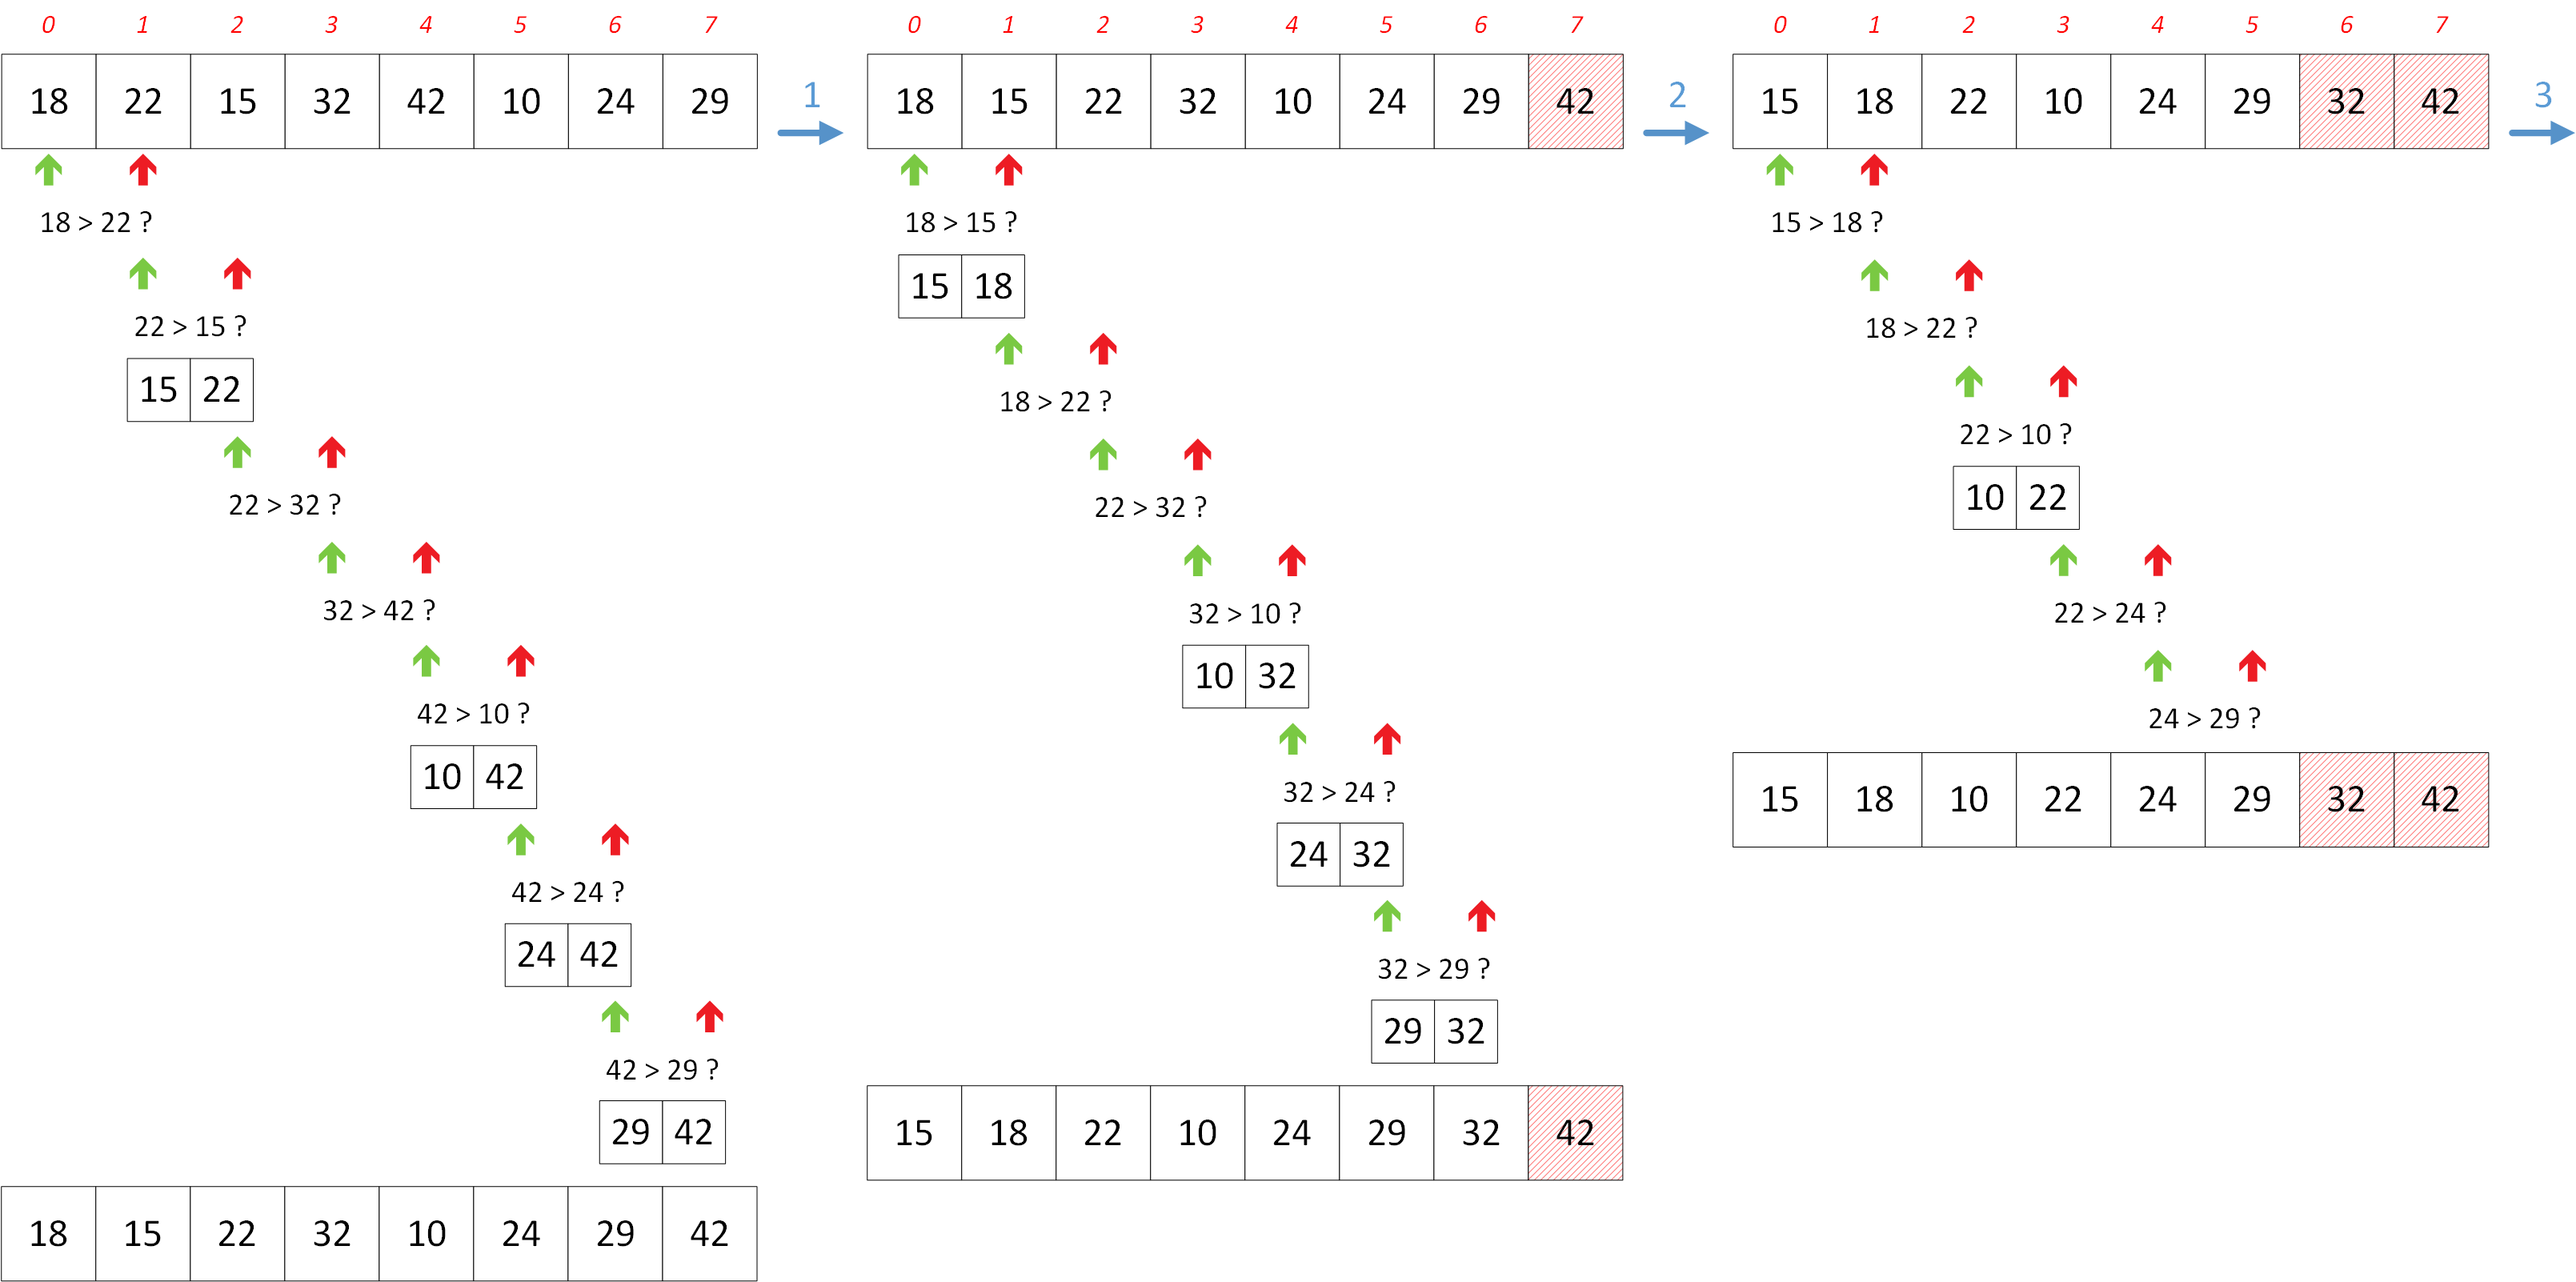
\includegraphics[width=1.2\textwidth]{img/BubbleSort_part1.png}
}
%\caption{Bubble Sort part 1}
%\label{figure:1-S3-DesignScience-ThreeLoops}
\end{figure}
%\end{figure*} % Figure flottante
% To use it : fig~\ref{label}

%\begin{figure*} % Figure flottante
\begin{figure}[ht!]
\centering
\centerline{
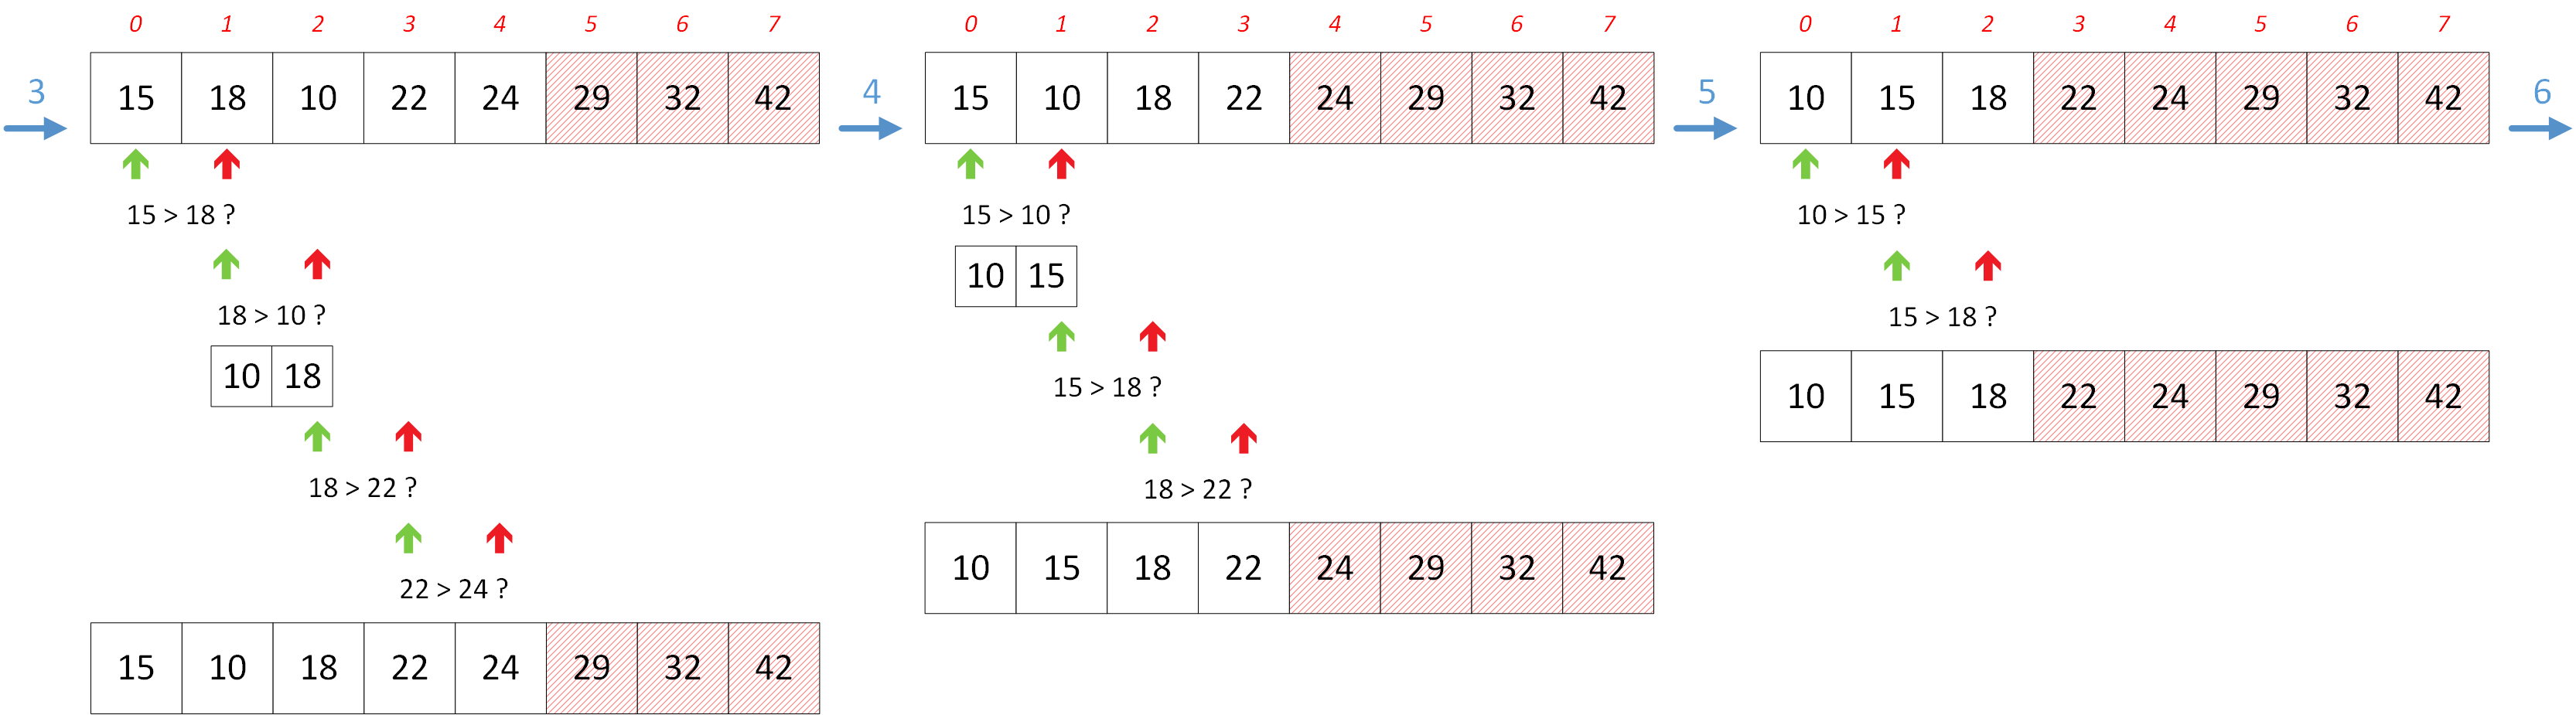
\includegraphics[width=1.2\textwidth]{img/BubbleSort_part2_1.png}
}
%\caption{Bubble Sort part 1}
%\label{figure:1-S3-DesignScience-ThreeLoops}
\end{figure}
%\end{figure*} % Figure flottante
% To use it : fig~\ref{label}


%\begin{figure*} % Figure flottante
\begin{figure}[ht!]
\centering
\centerline{
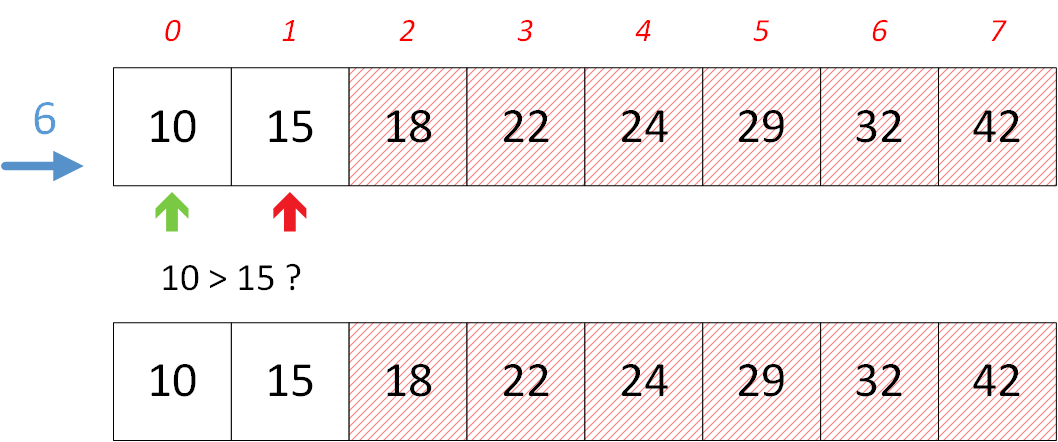
\includegraphics[scale=0.48]{img/BubbleSort_part2_2.png}
}
%\caption{Bubble Sort part 1}
%\label{figure:1-S3-DesignScience-ThreeLoops}
\end{figure}
%\end{figure*} % Figure flottante
% To use it : fig~\ref{label}


%\bigskip
\clearpage

\vfillFirst

\question{Écrivez une procédure de tri respectant l'algorithme du tri à bulles (ou \textit{bubble sort} en anglais). Vous devez modifier la position des éléments dans le tableau créer de tableau supplémentaire. \textit{BubbleSort(tab, len)} }

\begin{table}[ht!]
  \centering
% %*   *)
\begin{lstlisting}[style=algorithmique]
algorithme procedure BubbleSort
  parametres locaux
    entier[]  tab
    entier    len
  variables
    entier    i, j
debut
pour i = (len - 1) jusqu'a 1
  pour j = 0 jusqu'a (i - 1)
    si (tab[j] > tab[j + 1])
      swap(tab, len, j, j + 1)
    fin si
  fin pour
fin pour
fin algorithme procedure BubbleSort \end{lstlisting}
%  \caption{Bla. }
%  \label{puissance}
\end{table}


Dans cette version du Bubble Sort, on va chercher à pousser les plus gros éléments à la fin à chaque fois en faisant avancer chaque élément plus grand vers la droite.
Une fois que le plus grand élément a été trouvé, il est naturellement poussé vers la droite.
Une fois que ce plus grand élément est poussé à la fin du tableau, plus aucun élément ne sera plus grand, donc inutile de les comparer avec.
%Dans cette version du Bubble Sort, on va chercher à pousser les plus gros éléments à la fin à chaque fois en faisant avancer chaque élément plus grand vers la droite. Une fois que le plus grand élément a été trouvé, il est naturellement poussé vers la droite.
Ainsi, la dernière case la plus à droite devient immuable.
La première boucle avec i permet de déterminer quelle colonne va servir de fin pour les balayages successifs, et à chaque itération, on n'ira pas plus loin.
La boucle utilisant j permet d'effectuer les balayages successifs et d'échanger la position entre un élément courant et son suivant s'il est plus petit.
Ainsi, en tombant sur le plus grand élément, on va le déplacer progressivement jusqu'à la fin du tableau. On recommence avec les éléments restants, donc avec le 2e plus grand, et ainsi de suite.

\vfillLast

%\bigskip

\newpage


\subsection{Tri par sélection}

\bigskip

Le tri par sélection est le tri le plus évident humainement parlant : on cherche le plus grand élément dans le tableau en parcourant toutes les cases, puis, on échange la place de cet élément avec le tout dernier du tableau (pour le placer à sa place définitive).
On recommence ce traitement (sans lire la dernière case à chaque fois) jusqu'à avoir ordonné tous les éléments.

\vfillFirst

%\begin{figure*} % Figure flottante
\begin{figure}[ht!]
\centering
\centerline{
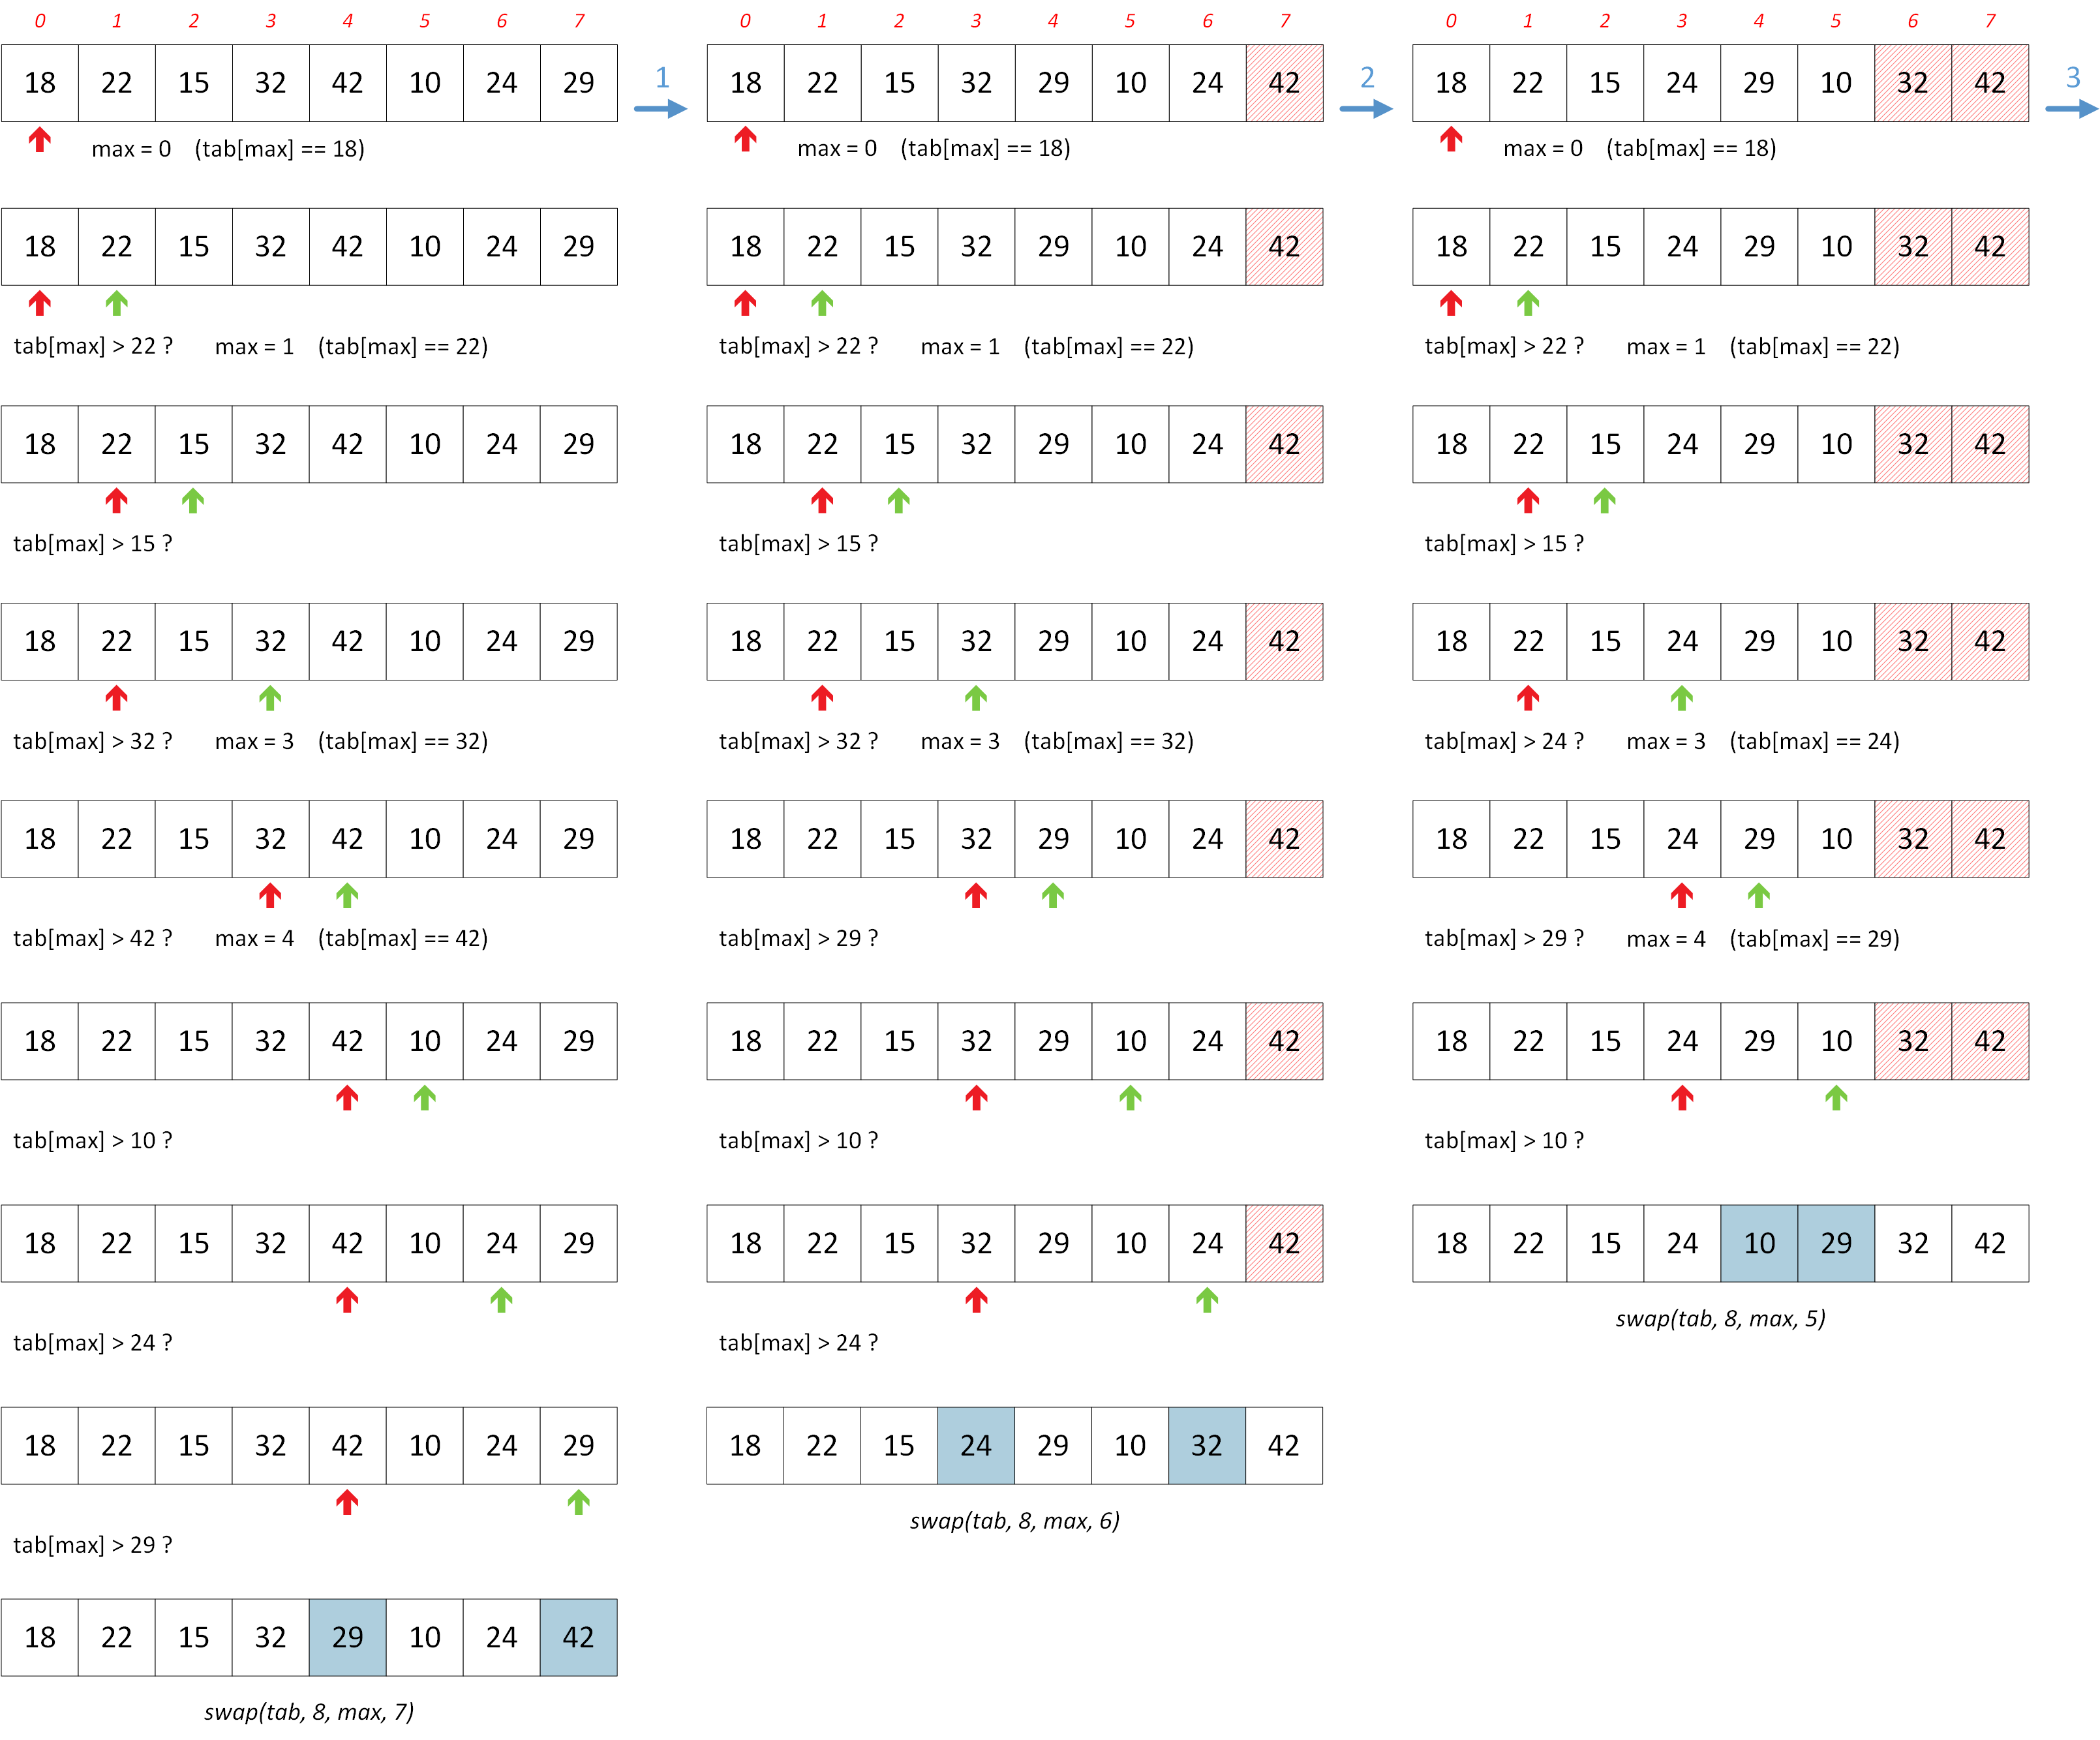
\includegraphics[width=1.2\textwidth]{img/SelectionSort_part1.png}
}
%\caption{Bubble Sort part 1}
%\label{figure:1-S3-DesignScience-ThreeLoops}
\end{figure}
%\end{figure*} % Figure flottante
% To use it : fig~\ref{label}

\vfillLast

\clearpage

\vfillFirst

%\begin{figure*} % Figure flottante
\begin{figure}[ht!]
\centering
\centerline{
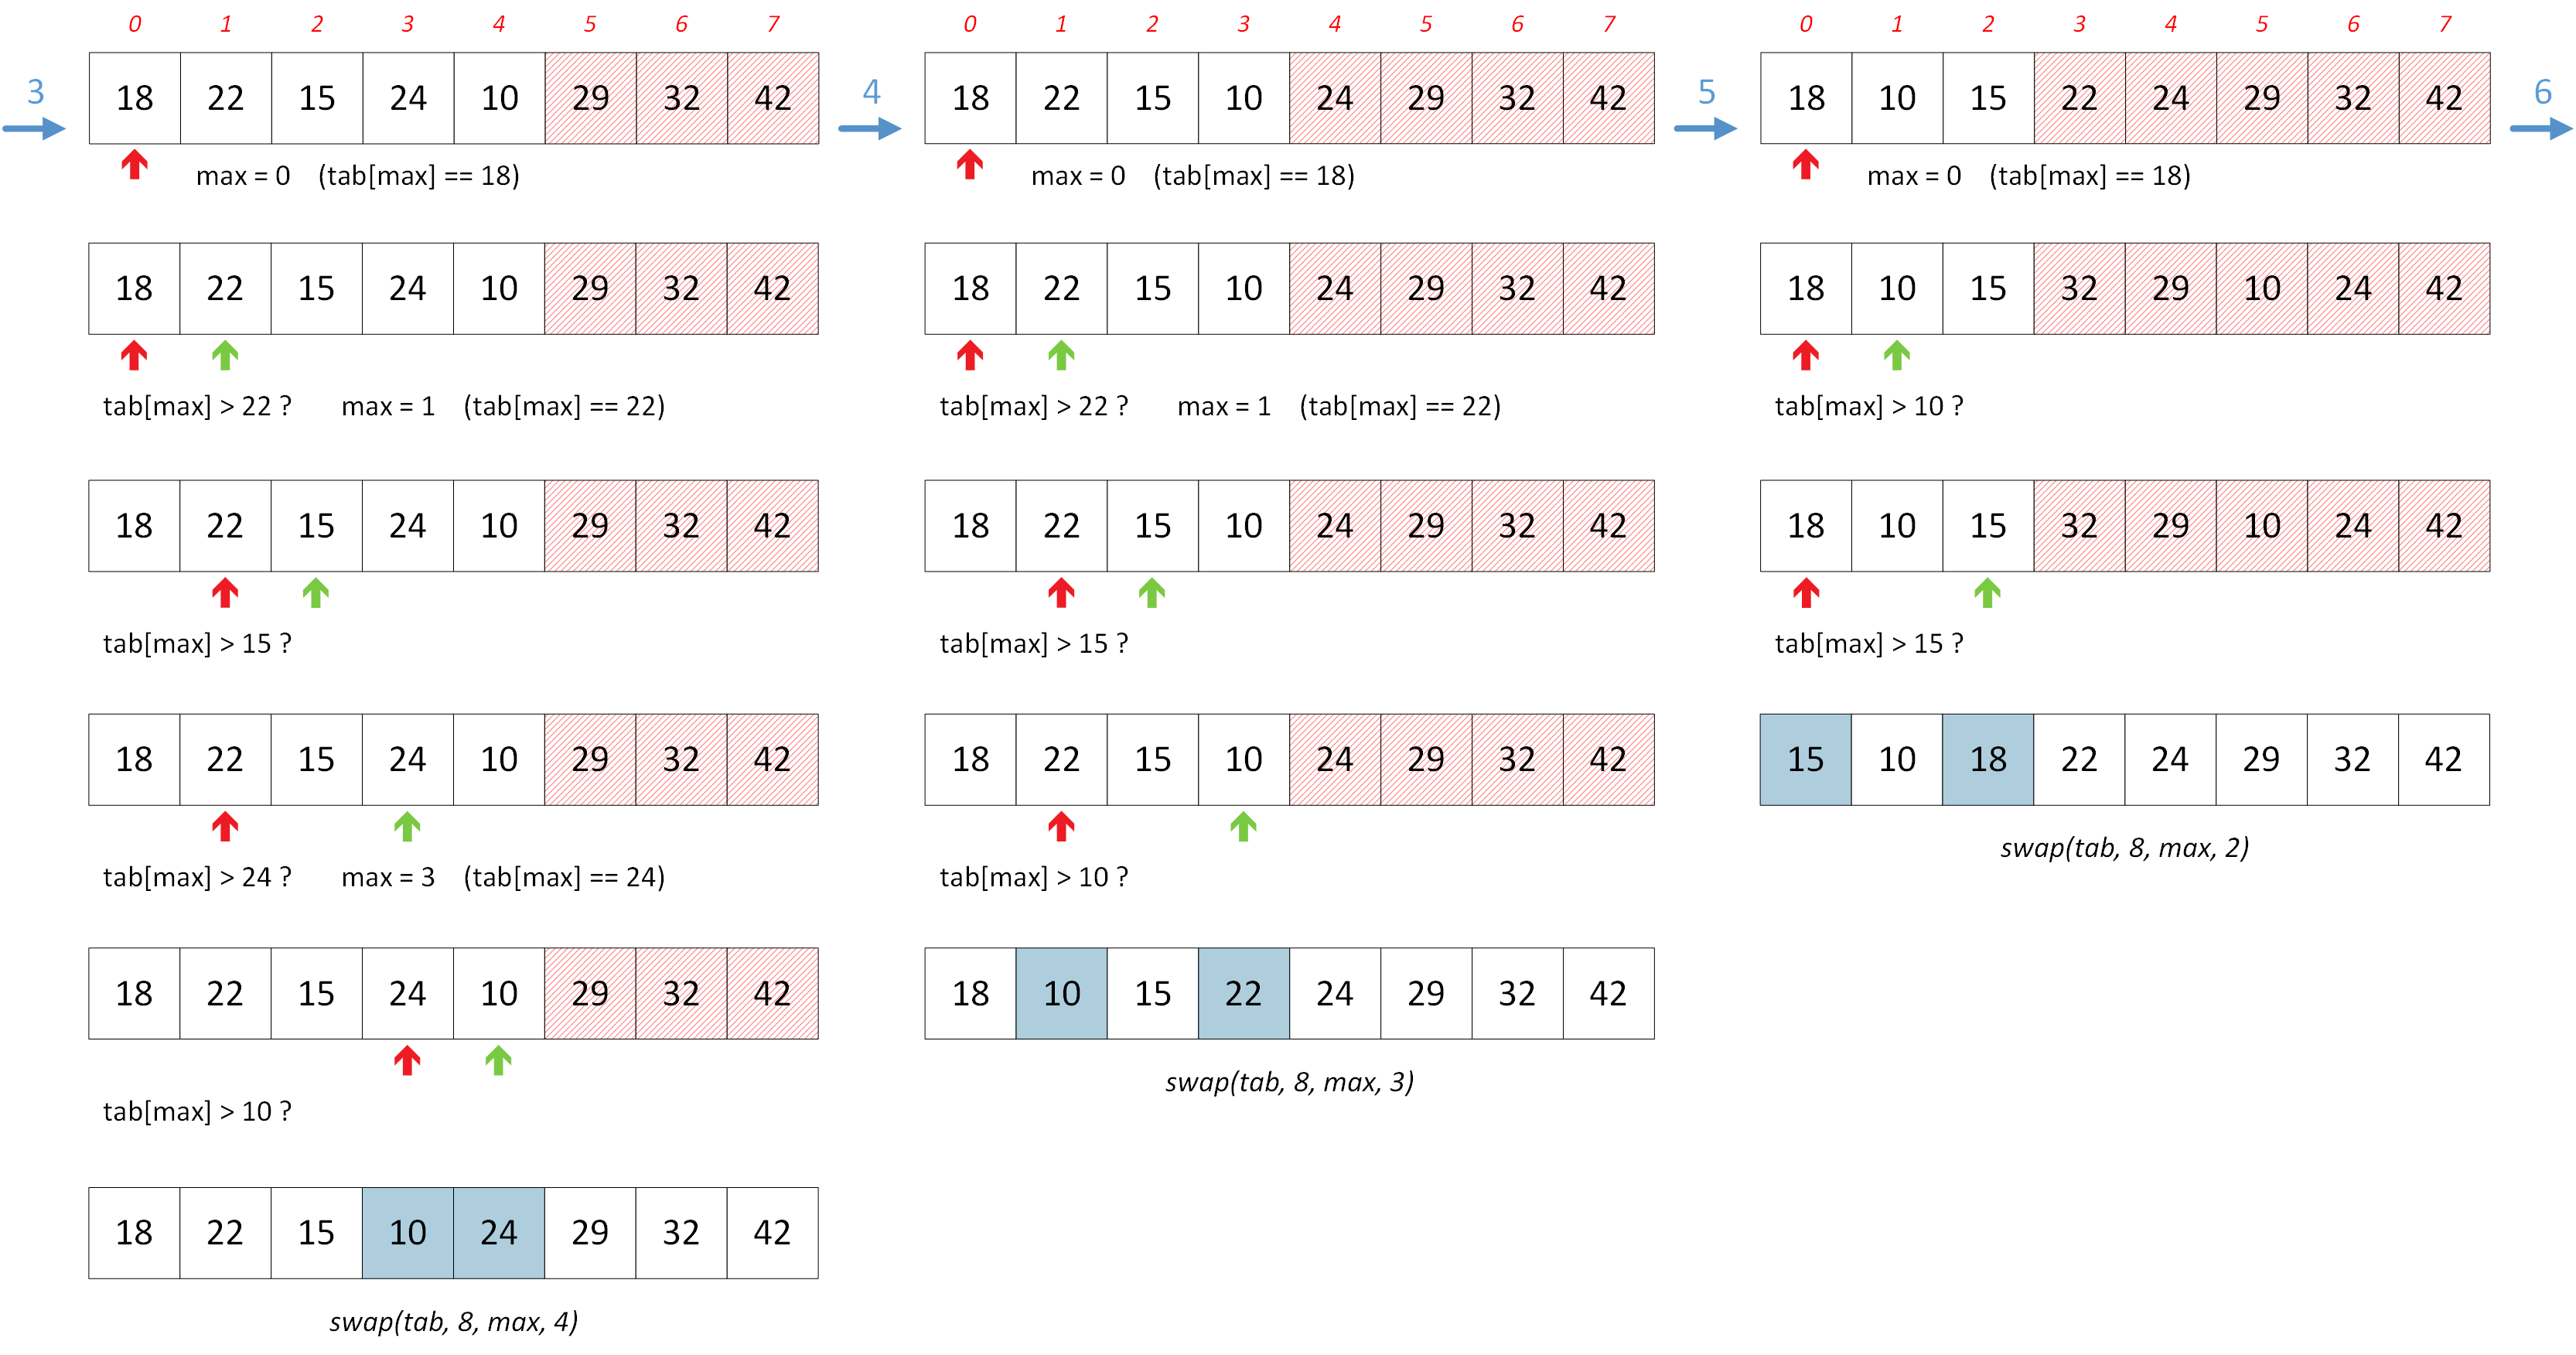
\includegraphics[width=1.2\textwidth]{img/SelectionSort_part2_1.png}
}
%\caption{Bubble Sort part 1}
%\label{figure:1-S3-DesignScience-ThreeLoops}
\end{figure}
%\end{figure*} % Figure flottante
% To use it : fig~\ref{label}

%\begin{figure*} % Figure flottante
\begin{figure}[ht!]
\centering
\centerline{
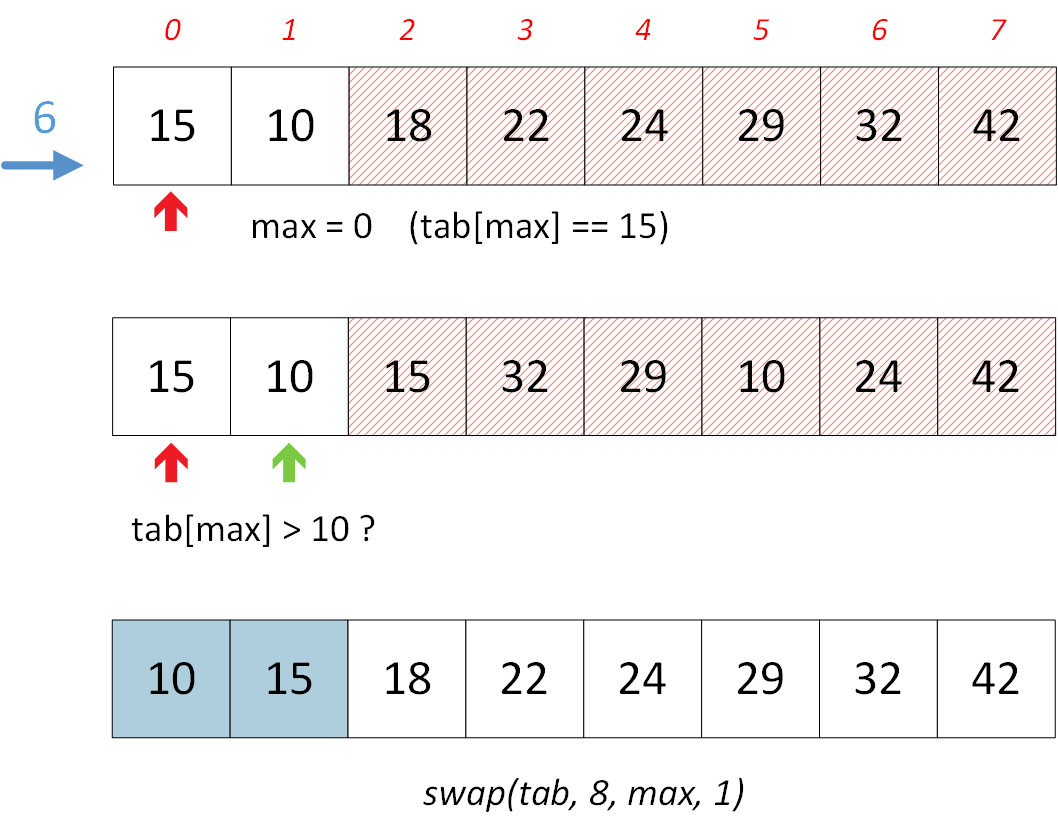
\includegraphics[scale=0.5]{img/SelectionSort_part2_2.png}
}
%\caption{Bubble Sort part 1}
%\label{figure:1-S3-DesignScience-ThreeLoops}
\end{figure}
%\end{figure*} % Figure flottante
% To use it : fig~\ref{label}

\vfillLast

%\bigskip
\clearpage

\question{Écrivez une procédure de tri respectant l'algorithme du tri par sélection (ou \textit{selection sort} en anglais). Vous devez modifier la position des éléments dans le tableau sans créer de tableau supplémentaire. \textit{SelectionSort(tab, len)} }

\begin{table}[ht!]
  \centering
% %*   *)
\begin{lstlisting}[style=algorithmique]
algorithme procedure SelectionSort
  parametres locaux
    entier[]  tab
    entier    len
  variables
    entier    max_range, max
debut
pour max_range = (len - 1) jusqu'a 2
  max = 0
  pour i = 1 jusqu'a (max_range)
    si (tab[i] > tab[max])
      max = i
    fin si
  fin pour
  swap(tab, len, max, max_range)
fin pour
fin algorithme procedure SelectionSort \end{lstlisting}
%  \caption{Bla. }
%  \label{puissance}
\end{table}

Cas général permettant de parcourir le tableau plusieurs fois.
\`A chaque parcours, on cherche la valeur la plus grande, et on la place à la fin.
\'Etant donné que le plus grand élément est placé en fin, on va réduire le parcours d'un élément à chaque fois.
Ainsi, le premier parcours fera la longueur du tableau, le dernier parcours ne fera que comparer les 2 premiers éléments pour placer correctement les deux plus petits éléments du tableau.

Cet algorithme a l'inconvénient de nécessiter au moins 3 éléments dans le tableau pour fonctionner correctement.
Ainsi, on peut soit faire une fonction chapeau testant les cas où la longueur est inférieure à 3, soit ajouter un pré-traitement dans la fonction.

\begin{table}[ht!]
  \centering
% %*   *)
\begin{lstlisting}[style=algorithmique]
algorithme procedure PreProcessingSelectionSort
  parametres locaux
    entier[]  tab
    entier    len
debut
si (len >= 2)
  si (len == 2)
    si (tab[0] > tab[1])
      swap(tab, len, 0, 1)
    fin si
  sinon
    SelectionSort(tab, len)
  fin si
fin si
fin algorithme procedure PreProcessingSelectionSort \end{lstlisting}
%  \caption{Bla. }
%  \label{puissance}
\end{table}

%\bigskip

\newpage


\subsection{Tri par insertion}

Le tri par insertion considère que le tableau donné en paramètre n'est pas trié, et seuls les éléments qu'il a manipulé successivement le sont.
Ainsi, chaque élément du tableau est comparé à tous ceux déjà triés, et on le place là où il devrait être.
Pour le premier élément, celui-ci est considéré comme déjà trié, on peut donc passer au deuxième.
Le deuxième est comparé avec l'unique élément déjà trié : on échange leurs deux places si nécessaire.
Le troisième élément est comparé au plus grand des deux éléments triés, s'il est plus grand ou égal, il reste à sa place, sinon on le décale vers la gauche d'un cran, et on le compare à l'élément suivant (et ainsi de suite).
Chaque élément du tableau est donc \textit{inséré} à sa place parmi les éléments considérés comme triés.

%\begin{figure*} % Figure flottante
\begin{figure}[ht!]
\centering
\centerline{
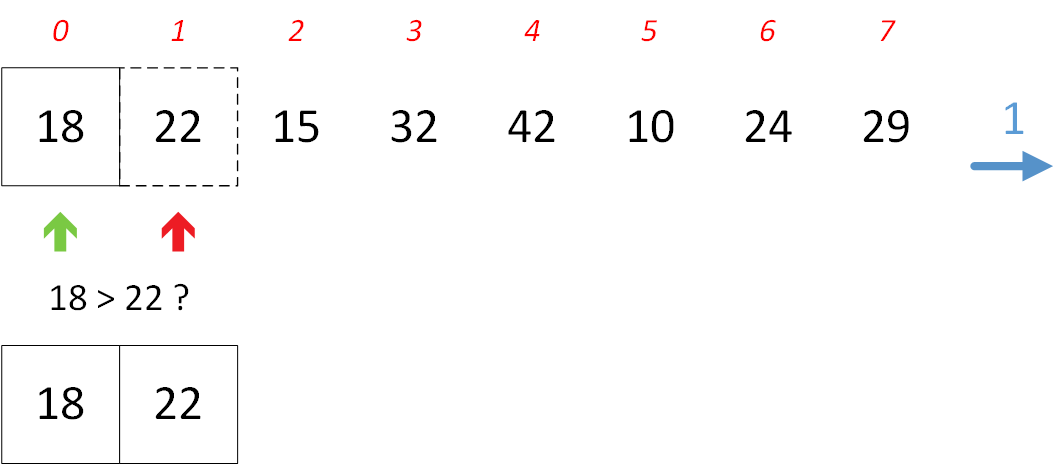
\includegraphics[scale=0.48]{img/InsertionSort_part1_1.png}
}
%\caption{Bubble Sort part 1}
%\label{figure:1-S3-DesignScience-ThreeLoops}
\end{figure}
%\end{figure*} % Figure flottante
% To use it : fig~\ref{label}

%\begin{figure*} % Figure flottante
\begin{figure}[ht!]
\centering
\centerline{
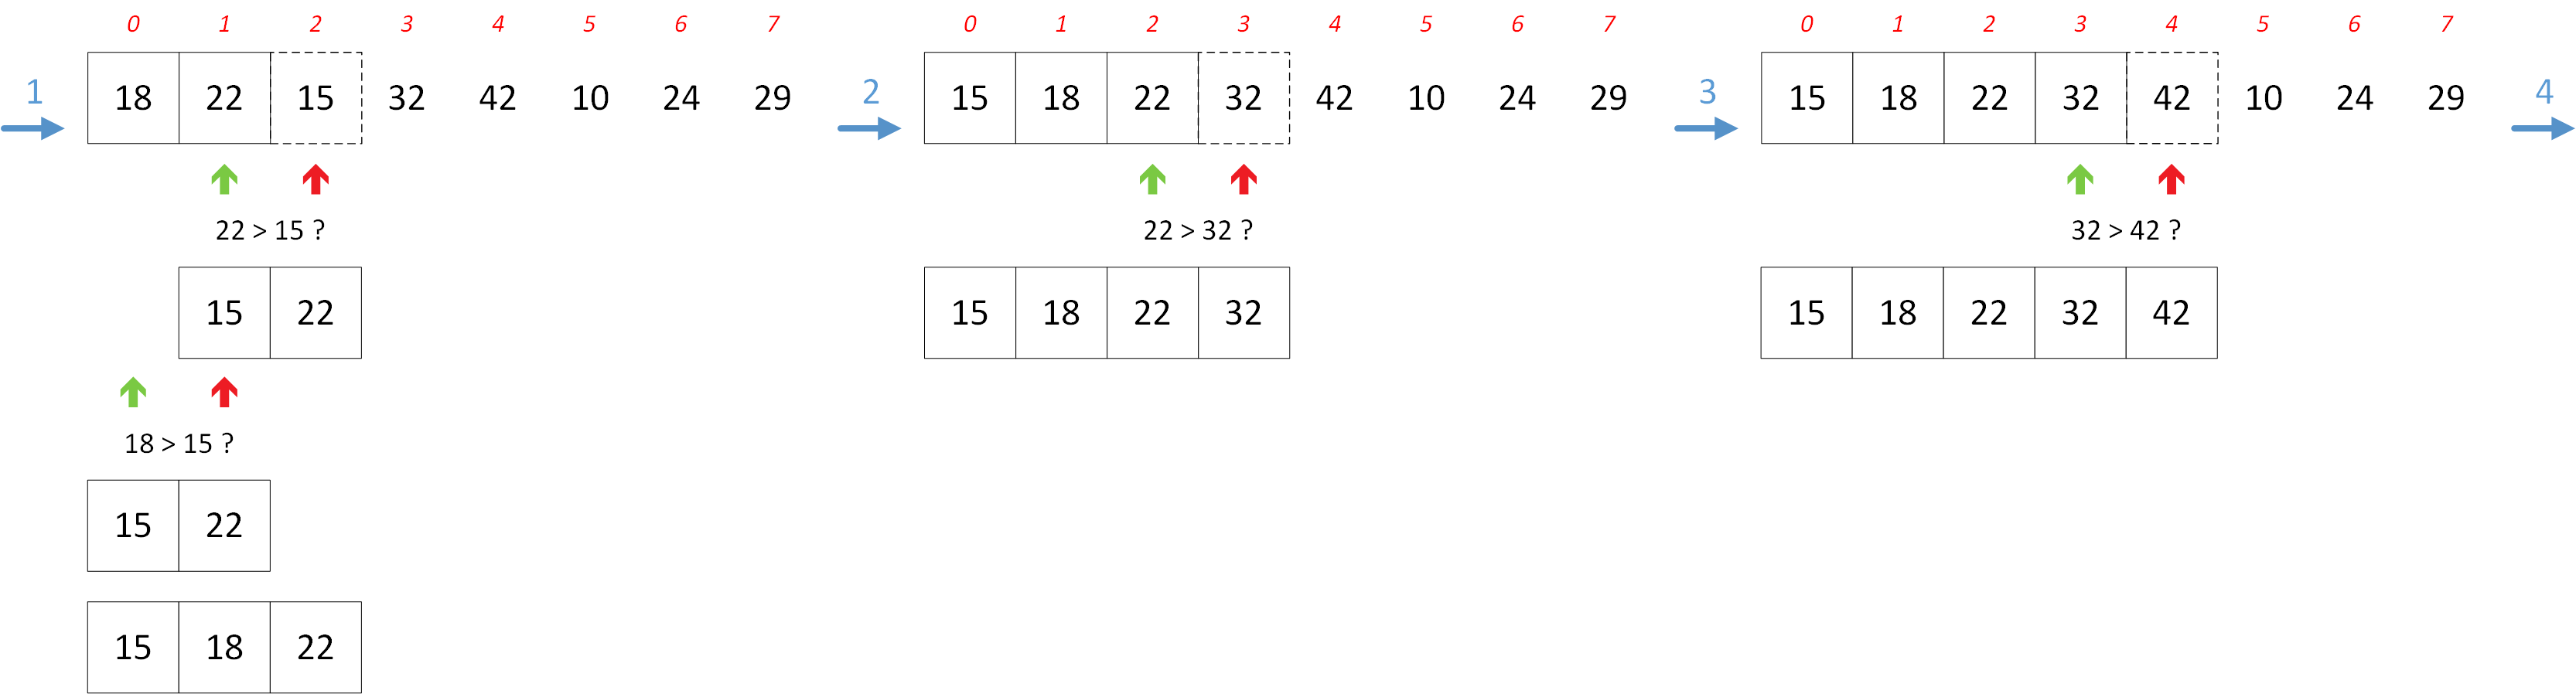
\includegraphics[width=1.18\textwidth]{img/InsertionSort_part1_2.png}
}
%\caption{Bubble Sort part 1}
%\label{figure:1-S3-DesignScience-ThreeLoops}
\end{figure}
%\end{figure*} % Figure flottante
% To use it : fig~\ref{label}

%\begin{figure*} % Figure flottante
\begin{figure}[ht!]
\centering
\centerline{
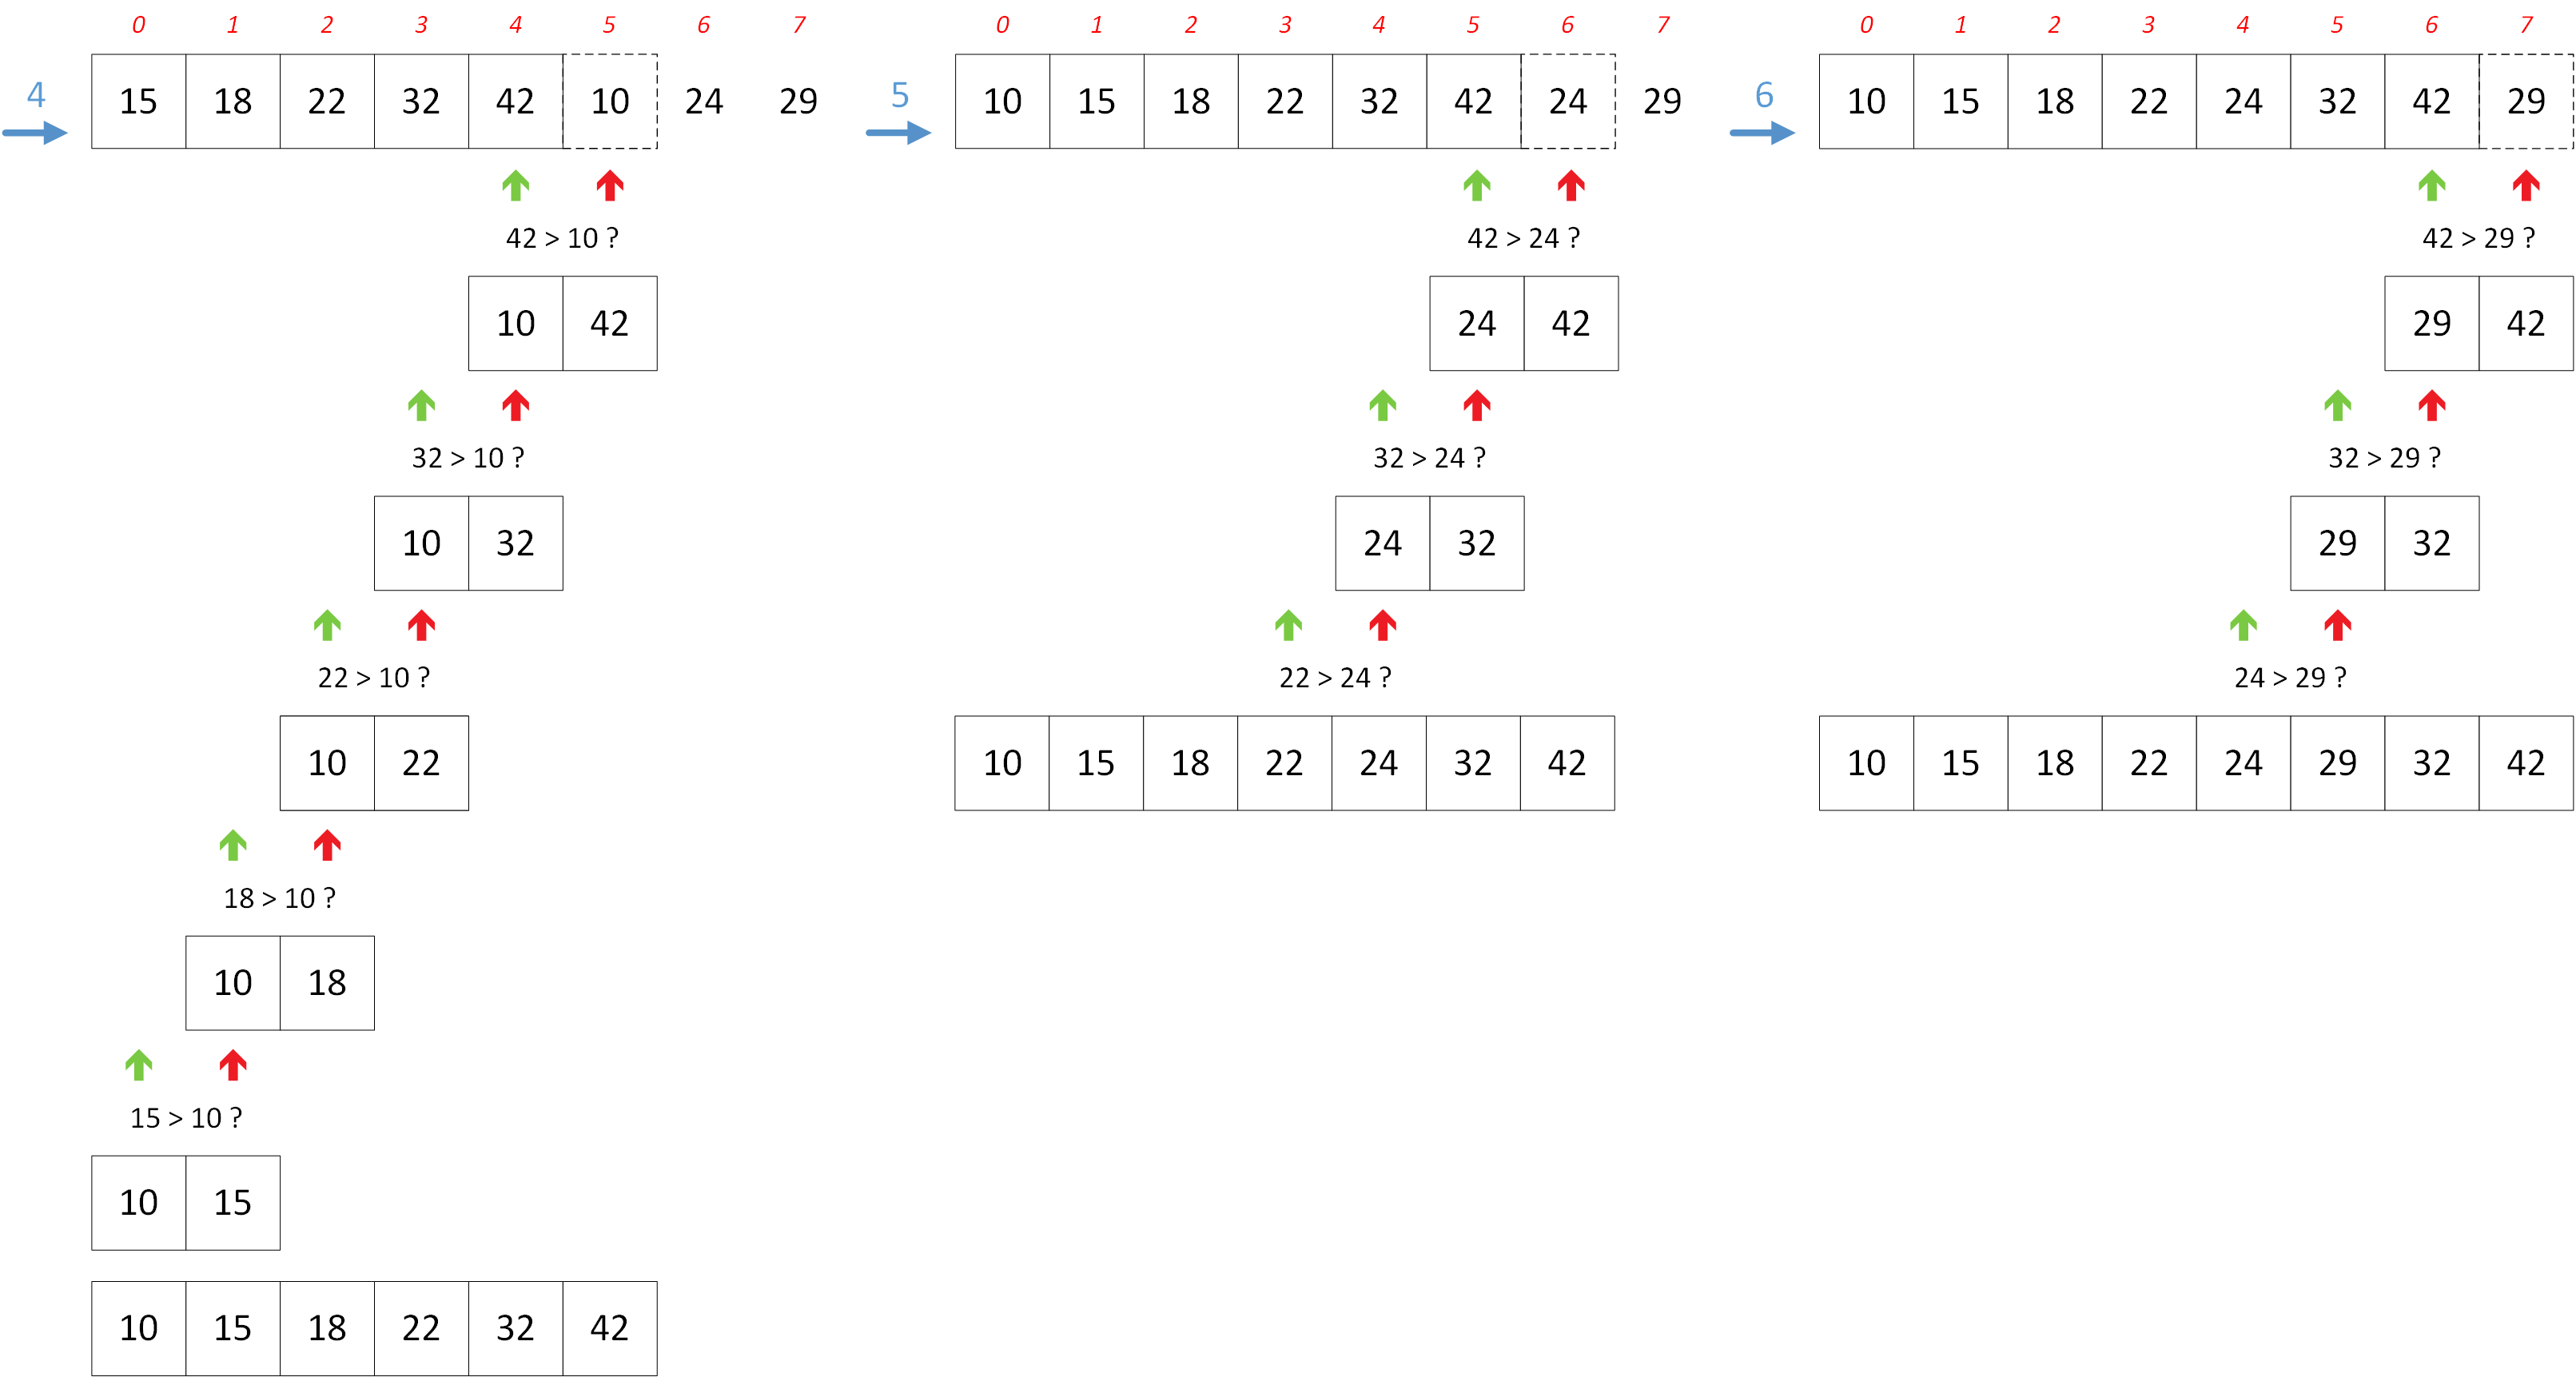
\includegraphics[width=1.18\textwidth]{img/InsertionSort_part2.png}
}
%\caption{Bubble Sort part 1}
%\label{figure:1-S3-DesignScience-ThreeLoops}
\end{figure}
%\end{figure*} % Figure flottante
% To use it : fig~\ref{label}

%\bigskip
\clearpage

\vfillFirst

\question{Écrivez une procédure de tri respectant l'algorithme du tri par insertion (ou \textit{insertion sort} en anglais). Vous devez modifier la position des éléments dans le tableau créer de tableau supplémentaire. \textit{InsertionSort(tab, len)} }


\begin{table}[ht!]
  \centering
% %*   *)
\begin{lstlisting}[style=algorithmique]
algorithme procedure InsertionSort
  parametres locaux
    entier[]  tab
    entier    len
  variables
    entier    max_range, elt
debut
pour max_range = 1 jusqu'a (len - 1)
  elt = max_range
  tant que (elt > 0) et (tab[elt] < tab[elt - 1])
    swap(tab, len, elt, (elt - 1))
    elt = elt - 1
  fin tant que
fin pour
fin algorithme procedure InsertionSort \end{lstlisting}
%  \caption{Bla. }
%  \label{puissance}
\end{table}


Cette fois, l'algorithme s'appuie sur l'idée que l'on va "insérer" des valeurs successivement.
Le tableau est en réalité déjà rempli, mais on va considérer qu'il est intégralement non-trié, et que l'on va petit à petit trier les éléments depuis le premier jusqu'au dernier.
Pour cela, on va "reconstruire" un tableau trié en déplaçant chaque élément à la place où il devrait être.
Le premier élément du tableau étant seul, il est donc trié.
On peut passer au deuxième élément et le comparer à l'unique élément déjà présent : doit-il être placé avant ou après le 1er élément ?
On échange éventuellement les places.
Ensuite, on peut passer au troisième élément : est-il plus grand ou plus petit que le deuxième ?
S'il est plus grand, il reste à sa place et on peut s'occuper du quatrième élément.
S'il est plut petit, on inverse leurs positions, et on se repose la question concernant le nouvel élément et le premier : lequel est le plus grand ?
Ainsi, on itère du 1er élément jusqu'au dernier, et on effectue tous les échanges nécessaires pour placer le nouvel élément au bon endroit.
Lorsque l'on analyse l'algorithme, on se rend compte que les éléments "avant" celui traité sont tous ordonnés, et les éléments "après" celui traité ne sont pas encore connus.

Comme pour le tri par sélection, on doit absolument avoir un tableau de trois éléments ou plus pour pouvoir exécuter cet algorithme.
Ainsi, on doit également ajouter un pré-traitement dans l'algorithme même, ou écrire une fonction chapeau.


%\begin{table}[ht!]
%  \centering
%% %*   *)
%\begin{lstlisting}[style=algorithmique]
%algorithme procedure PreProcessingInsertionSort
%  parametres locaux
%    entier[]  tab
%    entier    len
%debut
%si (len >= 2)
%  si (len == 2)
%    si (tab[0] > tab[1])
%      swap(tab, len, 0, 1)
%    fin si
%  sinon
%    InsertionSort(tab, len)
%  fin si
%fin si
%fin algorithme procedure PreProcessingInsertionSort \end{lstlisting}
%%  \caption{Bla. }
%%  \label{puissance}
%\end{table}

\vfillLast



\begin{center}
\textit{Ce document et ses illustrations ont été réalisés par Fabrice BOISSIER en octobre 2022.\\
La plupart des exercices sont inspirés du cahier d'algo de Nathalie "Junior" BOUQUET et Christophe "Krisboul" BOULLAY.}
\end{center}

\end{document}
